\documentclass[a4paper,11pt]{report}
\usepackage{amsmath}
\usepackage{amsfonts}
\usepackage{amssymb}
\usepackage{float}
\newcommand{\di}{\displaystyle}
\def\rmm{\rm}
\newcommand{\goth}{\mathfrak}
\newcommand{\be}{\begin{eqnarray}}
\newcommand{\ee}{\end{eqnarray}}
\newcommand{\bee}{\begin{eqnarray*}}
\newcommand{\eee}{\end{eqnarray*}}
\newcommand{\RR}{\Bbb{R}}
\newcommand{\NN}{\Bbb{N}}
\newcommand{\CC}{\Bbb{C}}
\newcommand{\ZZ}{\Bbb{Z}}
\newcommand{\Gal}{{\rmm Gal}}
\newcommand{\mean}{\mathop{\rmm mean}}
\newcommand{\Ad}{{\rmm Ad}}
\newcommand{\Area}{{\rmm Area}}
\newcommand{\pr}{{\rmm pr}}
\newcommand{\tr }{{\rmm tr }}
\newcommand{\Int}{{\rmm Int}}
\newcommand{\Ext}{{\rmm Ext}}
\newcommand{\Vol}{{\rmm Vol}}
\newcommand{\Inn}{{\rmm Inn}}
\newcommand{\Aut}{{\rmm Aut }}
\newcommand{\Ker}{{\rmm Ker }}
\newcommand{\Hom}{{\rmm Hom }}
\newcommand{\Mat}{{\rmm Mat }}
\newcommand{\rank}{{\rmm rank }}
\newcommand{\sgn}{{\rmm sgn }}
\newcommand{\Real}{{\rmm Re }}
\newcommand{\Image}{{\rmm Im }}
\newcommand{\arccot}{{\rmm arccot}}
\newcommand{\arcsec}{{\rmm arcsec}}
\newcommand{\arccsc}{{\rmm arccsc}}
\newcommand{\sech}{{\rmm sech}}
\newcommand{\csch}{{\rmm csch}}
\newcommand{\arcsinh}{{\rmm arcsinh}}
\newcommand{\arcsech}{{\rmm arcsech}}
\newcommand{\arccsch}{{\rmm arccsch}}
\newcommand{\arctanh}{{\rmm arctanh}}
\newcommand{\arccoth}{{\rmm arccoth}}
\newcommand{\Dri}{{\rmm Dri}}
\newcommand{\proj}{{\rmm proj}}
\newcommand{\Char}{{\rmm Char}}
\newcommand{\Beta}{{\rmm B }}
\newcommand{\divv}{{\rmm div }}
\newcommand{\Curl}{{\rmm Curl }}
\newcommand{\PSL}{{\rmm PSL }}
\newcommand{\BSA}{{\rmm BSA }}
\newcommand{\Span}{{\rmm Span}}
\newcommand{\GL}{{\rmm GL }}
\newcommand{\SE}{{\rmm SE }}
\newcommand{\SL}{{\rmm SL }}
\newcommand{\SO}{{\rmm SO }}
\newcommand{\SA}{{\rmm SA }}
\newcommand{\pa}{\paragraph}
\newcommand{\1}{{\rmm 1}}
\newcommand{\esbat}{\medskip \noindent {\it اثبات:} }
%

%
%\newcommand{\listoftables}{\listoftables}
%\setlength{\evensidemargin}{0mm}
%\setlength{\oddsidemargin}{0mm}
%\setlength{\textwidth}{16cm}
%\setlength{\textheight}{23cm}
%\setlength{\headsep}{1cm}
%\setlength{\topmargin}{0mm}
%\setlength{\columnsep}{1.5cm}

\makeindex                %    < این فایل شامل دستوراتی برای نمادگذاری‌های می‌باشد آن‌ها استفاده کرد>
% در این فایل، دستورها و تنظیمات مورد نیاز، آورده شده است.
%-------------------------------------------------------------------------------------------------------------------

\usepackage{booktabs}
% در ورژن جدید زی‌پرشین برای تایپ متن‌های ریاضی، این سه بسته، حتماً باید فراخوانی شود
\usepackage{amsthm,amssymb,amsmath}
% بسته‌ای برای تنطیم حاشیه‌های بالا، پایین، چپ و راست صفحه
\usepackage[top=40mm, bottom=35mm, left=25mm, right=30mm]{geometry}
% بسته‌‌ای برای ظاهر شدن شکل‌ها و تصاویر متن
\usepackage{graphicx,textpos}
\usepackage[usenames,dvipsnames]{color}
\usepackage{xcolor,listings}
%\usepackage{hyperref} 							% 	PDF links
\usepackage{setspace} 				    		% 	for switching between double/single space in document
\graphicspath{{images}}
\usepackage{verbatim}

\usepackage{natbib}                             %   برای ظاهر شدن مراجع فارسی درصورت استفاده از بیب فایل%
                                              
                    %  براي ارجاعات با پرانتز سطر فوق را فعال كرده و سطر زير را غير فعال كنيد.
%\usepackage[nonamebreak,square]{natbib}%nonamebreak,numbers,

%\usepackage{tocbibind}  % بسته‌ای برای ظاهر شدن «مراجع» و «نمایه» در فهرست مطالب

% بسته‌ای برای رسم کادر
\usepackage{framed} 
% بسته‌‌ای برای چاپ شدن خودکار تعداد صفحات در صفحه «معرفی پایان‌نامه»
\usepackage{lastpage}
% بسته‌‌ای برای ایجاد دیاگرام‌های مختلف
\usepackage[all]{xy}
% بسته‌ و دستوراتی برای ایجاد لینک‌های رنگی با امکان جهش
\usepackage[pdfmenubar=true,pagebackref=false,colorlinks=true,linkcolor=blue,citecolor=magenta,linktoc=none]{hyperref}
% چنانچه قصد پرینت گرفتن نوشته خود را دارید، خط بالا را غیرفعال و  از دستور زیر استفاده کنید چون در صورت استفاده از دستور زیر‌‌، 
% لینک‌ها به رنگ سیاه ظاهر خواهند شد که برای پرینت گرفتن، مناسب‌تر است
%\usepackage[pagebackref=false]{hyperref}
% بسته‌ لازم برای تنظیم سربرگ‌ها
\usepackage{fancyhdr}
% بسته‌ای برای ظاهر شدن «مراجع» و «نمایه» در فهرست مطالب
\usepackage[nottoc]{tocbibind}
% دستورات مربوط به ایجاد نمایه
\usepackage{makeidx}
\makeindex
 
                                       %دستوری برای ایجاد زیر بخش‌های تودرتو همراه با شماره در فهرست
\setcounter{secnumdepth}{4}
\setcounter{tocdepth}{4} 
\usepackage{textcomp}         %بسته‌ای برای غیر قابل کپی برداری شدن فایل پی دی اف
%%%%%%%%%%%%%%%%%%%%%%%%%%
 %                                                       ---------------------------------------------------------		
 	                                      %   فراخوانی بسته زی‌پرشین و تعریف قلم فارسی و انگلیسی %
 	                                                             %XePersian  دستورات مربوط به 
\usepackage{xepersian}
\settextfont[Scale=1.15]{B Nazanin}
\setdigitfont[Scale=1]{Times New Roman}
\setlatintextfont{Times New Roman}
\defpersianfont\minutesfont[Scale=1.2]{B Nazanin}			        
% 																	-------------------------------------
% از revision 118 زی‌پرشین به بعد، وارد کردن دستور زیر لازم نیست. توجه داشته باشید که در صورت  غیرفعال کردن این %دستور،
% از فونت پیش‌فرض لاتک برای کلمات انگلیسی استفاده خواهد شد.
%%%%%%%%%%%%%%%%%%%%%%%%%%
% چنانچه می‌خواهید اعداد در فرمول‌ها، انگلیسی نباشد، خط زیر را غیرفعال کنید
%\DefaultMathDigits
%%%%%%%%%%%%%%%%%%%%%%%%%%
% تعریف قلم‌های فارسی و انگلیسی اضافی برای استفاده در بعضی از قسمت‌های متن
\defpersianfont\nastaliq[
Scale=2,
Script=Arabic,
BoldFont=IranNastaliq,
BoldFeatures={FakeBold=1},]{IranNastaliq}
\defpersianfont\chapternumber[
Scale=1.5,
BoldFont=B Nazanin,
BoldFeatures={FakeBold=1}]{B Nazanin}
\defpersianfont\titr[
Scale=1,
BoldFont=B Nazanin,
BoldFeatures={FakeBold=1}]{B Nazanin}
\settextfont{Persian Modern}
%%%%%%%%%%%%%%%%%%%%%%%%%%
%
%% دستوری برای حذف کلمه «چکیده»
%\renewcommand{\abstractname}{}
%% دستوری برای حذف کلمه «abstract»
%\renewcommand{\latinabstract}{}
% دستوری برای تغییر نام کلمه «اثبات» به «برهان»
\renewcommand\proofname{\textbf{برهان}}
% دستوری برای تغییر نام کلمه «کتاب‌نامه» به «مراجع»

\renewcommand{\bibname}{مرجع‌ها}
%دستوری برای اینکه لیست جدول و شکل به فهرست تبدیل شود:
\def\listfigurename{\if@RTL List of Figures \else فهرست‌ شکل‌‌ها \fi}
\def\listtablename{\if@RTL List of Tables ‌\else  فهرست جدول‌ها\fi}
% دستوری برای تعریف واژه‌نامه انگلیسی به فارسی
\newcommand\persiangloss[2]{#1\hfill\lr{#2}\\}
% دستوری برای تعریف واژه‌نامه فارسی به انگلیسی 
\newcommand\englishgloss[2]{#2\dotfill\lr{#1}\\}
%%%%%%%%%%%%%%%%%%%%%%%%%
\newcommand{\blockmatrix}[3]{%These end of the line comments are neccessary
\begin{minipage}[t][#2][c]{#1}%
\center%
#3%
\end{minipage}%
}%
\newcommand{\fblockmatrix}[3]{%
\fbox{%
\begin{minipage}[t][#2][c]{#1}%
\center%
#3%
\end{minipage}%
}%
}

%%%%%%%%%%%%%%%%%%%%%%%%%%
% تعریف و نحوه ظاهر شدن عنوان قضیه‌ها، تعریف‌ها، مثال‌ها و ...
\newtheorem{theo}{قضیه}[section]
\renewcommand{\thetheo}{\arabic{theo}.\arabic{section}.\arabic{chapter}}
\newcommand{\mored}[2]{{\large \theo{\bf #2.} \label{#1}}}
\newtheorem{lem}{لم}[section]
\renewcommand{\thelem}{\arabic{lem}.\arabic{section}.\arabic{chapter}}
%\newcommand{\mored}[2]{{\large \lem{\bf #2.} \label{#1}}}
\newtheorem{example}{مثال}[section]
%\renewcommand{\theexample}{\arabic{example}.\arabic{section}.\arabic{chapter}}
%\newcommand{\mored}[2]{{\large \example{\bf #2.} \label{#1}}}

\theoremstyle{definition}
\newtheorem{definition}{تعریف}[section]
%\theoremstyle{theorem}
%\newtheorem{theorem}[theo]{قضیه}
%\newtheorem{lemma}[theo]{لم}
\newtheorem{proposition}[theo]{گزاره}
\newtheorem{corollary}[definition]{نتیجه}
\newtheorem{remark}[definition]{ملاحظه}
%\theoremstyle{definition}
%\newtheorem{example}[definition]{مثال}
%%%%%%%%%%%%%%%%%%%%%%%%%%
% تعریف دستورات جدید برای خلاصه نویسی و راحتی کار در هنگام تایپ فرمول‌های ریاضی
\newcommand{\bR}{\mathbb{R}}
\newcommand{\cB}{\mathcal{B}}
\newcommand{\cO}{\mathcal{O}}
\newcommand{\cG}{\mathcal{G}}
\newcommand{\cU}{\mathcal{U}}
\newcommand{\cK}{\mathcal{K}}
\newcommand{\cS}{\mathcal{S}}
\newcommand{\rM}{\mathrm{M}}
\newcommand{\rC}{\mathrm{C}}
\newcommand{\rV}{\mathrm{V}}
\newcommand{\ls}{\mathrm{LSC}_{+}(X)}
\newcommand{\ce}{\mathrm{C}^{*}(X)}
\newcommand{\lsc}{\mathrm{LSC}}
\newcommand{\fB}{\mathfrak{B}}
\newcommand{\fM}{\mathfrak{M}}
\newcommand{\bt}{\begin{theorem}}
\newcommand{\et}{\end{theorem}}
\newcommand{\bl}{\begin{lemma}}
\newcommand{\el}{\end{lemma}}
\newcommand{\bc}{\begin{corollary}}
\newcommand{\ec}{\end{corollary}}
\newcommand{\bp}{\begin{proof}}
\newcommand{\ep}{\end{proof}}
%%%%%%%%%%%%%%%%%%%%%%%%%%%%
% دستورهایی برای سفارشی کردن سربرگ صفحات
\csname@twosidetrue\endcsname
\pagestyle{fancy}
\setlength{\headheight}{16pt}
\fancyhf{} 
\fancyhead[OL,EL]{\thepage}
\fancyhead[OR]{\small\rightmark}
\fancyhead[ER]{\small\leftmark}
\renewcommand{\chaptermark}[1]{%
\markboth{\thechapter.\ #1}{}}
%%%%%%%%%%%%%%%%%%%%%%%%%%%%%

% دستورهایی برای سفارشی کردن صفحات اول فصل‌ها
\makeatletter
\def\@makechapterhead#1{%
   \vspace*{-30\p@}% default: 50pt
   {\parindent \z@ %\raggedleft \normalfont% default: \raggedright
     \ifnum \c@secnumdepth >\m@ne
      \begin{flushleft}   
         \huge\bfseries \@chapapp\space \thechapter
         \par\nobreak
         \vskip 20\p@% default: 20\p@
     \fi
     \interlinepenalty\@M
     \Huge \bfseries #1\par\nobreak
     \vskip 120\p@
     \end{flushleft}
   }}
 \makeatother
 
               % <در این فایل، دستورها و تنظیمات مورد نیاز، آورده شده است>
%
% 
%		این اطلاعات را وارد نموده، ذخیره کنید و سپس فایل اصلی پایان نامه را اجرا کنید
% %-------------------------------------------------------------------------------------------------------------------
%		مشابه عنوان زیر، عنوان پایان نامه اضافه شود
\newcommand{\fatitle}{
	سطر اول عنوان پایان نامه
	\vskip0.4cm
	سطر دوم عنوان پایان نامه
}		
	
	                                                            %		نام و نام خانوادگی دانشجو اضافه شود		
\newcommand{\faAuthor}{نام پژوهشگر}			
                                                                 %		شماره دانشجو اضافه شود
\newcommand{\stuno}{شماره دانشجویی}
                                                                   %		نام و نام خانوادگی استاد راهنما اضافه شود
\newcommand{\fasupervisor}{ نام استاد راهنما}		
                                                                 %       نام و نام خانوادگی استاد مشاور اضافه شود    
\newcommand{\faadvisor}{نام استاد مشاور} 			
                                                                    %       نام و نام خانوادگی استاد داور اضافه شود         
\newcommand{\referee}{نام داور}                  
%		نام و نام خانوادگی نماینده تحصیلات تکمیلی راهنما اضافه شود%
%\newcommand{\representative}{نام و نام خانوادگی نماینده تحصیلات تکمیلی}



\newcommand{\fadate}{زمستان ۱۴۰۲}			  	%		در جای --- ماه و سال جلسه برگزاری دفاع از رساله اضافه شود
%
\newcommand{\fauniversity}{\vskip-0.1cm{\nastaliq  دانشگاه علامه طباطبائی }}
\newcommand{\fadepart}{\vskip-0.1cm{\nastaliq دانشکده آمار، ریاضی و رايانه}}
\vskip1cm
\newcommand{\falevel}{ پایان‌نامه کارشناسی ارشد }
\newcommand{\famajor}{ رشته علم داده‌ها }
\vskip-2cm
%------------------------------------------------------------------------------------------------------------------------------
                                                       %            در جای --- عنوان پایان نامه به صورت لاتین اضافه شود%
\newcommand{\entitle}{\LARGE FIRST LINE OF TITLE 
	\vskip0.2cm SECOND LINE OF TITLE
}				
\newcommand{\enAuthor}{your name}%در جای --- نام و نام خانوادگی دانشجو به صورت لاتین اضافه شود
\newcommand{\ensupervisor}{name of your supervisor}			%		در جای --- نام و نام خانوادگی استاد راهنما به صورت لاتین 
\newcommand{\enadvisor}{name of your enadvisor}                                  %جای --- نام و نام خانوادگی استاد مشاور به صورت لاتین
\newcommand{\enreferee}{name of your enreferee }                                  %جای --- نام و نام خانوادگی استاد داور به صورت لاتین
\newcommand{\engdate}{ُُwinter 2024}					%		در جای --- ماه و سال جلسه برگزاری دفاع از رساله به صورت لاتین اضافه شود
\newcommand{\enuniversity}{Allameh Tabataba'i University}
%   سطر زیر را متناسب با رشته تحصیلی تغییر دهید.
\newcommand{\enmajor}{Department of Statistics }
\newcommand{\enlevel}{ Thesis Submitted in Partial Fulfillment for the Degree of Master of Science (MSC) in the Data Science
}
\newcommand{\enDep}{Faculty of Statistics, Mathematics and Computer }
%-------------------------------------------------------------------------------------------------------------------
\newcommand{\momtahenina}{دکتر }  
\newcommand{\momtaheninb}{دکتر }   	
\newcommand{\momtaheninc}{دکتر }  	%    در جای --- اسامی 
%\newcommand{\momtahenoud}{دکتر } 
%\newcommand{\momtahenoue}{دکتر}   		%    در جای --- اسامی ممتحنین خارجی اضافه شود				 %		< به این فایل بروید و تغییرات لازم را انجام بدهید >
%
%---------------------------------------------------------------------

\begin{document}
\renewcommand{\bibname}{مرجع‌ها}
%
%
%                                                        توجه      توجه          توجه      توجه    
%											در این فایل تغییر نیاز نیست بدهید، 
%
%
%-------------------------------------------------------------------------------------------------------------------------------------------
\begin{center}
\thispagestyle{empty}

\includegraphics[width=25mm]{enatu.jpg} \\
\fauniversity
\fadepart \\[.5cm]
\begin{large}
\large \falevel \\[.5cm]
\textbf{\large\famajor}
\end{large}
\vskip .7cm
\large{عنوان}
\\
\vskip0.4cm
\textbf{\huge\fatitle  }

\vskip .8cm
\large{استاد راهنما}
\\
\vskip0.4cm
\Large{\fasupervisor}
\vskip .6cm
\large{استاد مشاور}
\\
\vskip0.4cm
\Large{\faadvisor}
\vskip .6cm
\large{استاد داور}
\\
\vskip0.4cm
\Large{\referee}
\vskip .8cm
\large{پژوهش‌گر}
\\
\vskip0.4cm
\Large{\faAuthor}
\vskip .6cm
{\normalsize \fadate}
\end{center}									%		صفحه اول به فارسی

%                                                                               توجه                
           %                                           این صفحه نیاز به تغییرات ندارد
%---------------------------------------------------------------------------------------------------------------------------------------
\newpage
\thispagestyle{empty}
\begin{center}
\begin{figure}[!h]
\centerline{
\includegraphics[height=15cm,width=12cm]{besme.pdf}} 
\end{figure}
\end{center}
% در صورت تمایل دستور زیر را فعال کنید.
%\begin{center} \Large 
%{\vskip-0.1cm{\nastaliq  بنام بخشایشگر مهربان }}
%\end{center}

\vfill

\mbox{ }

\newpage
\thispagestyle{empty}
  \vspace{5cm}
  \begin{center}
\begin{table}[ht]
\vspace{0.2cm}
\begin{center}
\begin{tabular}[c]{|c |}
\hline
\hline  
\\  
\\
\\
\textbf{کلیه‌ی حقوق مادی و معنوی اعم از چاپ و تکثیر، نسخه‌برداری، ترجمه، اقتباس و ... از این پایان‌نامه} 
 \\
 \\
 \\
 \textbf{برای دانشگاه علامه طباطبائی محفوظ است. 
  نقل مطالب با ذکر منبع مانعی ندارد.}    \\
    \\
    \\
    \\
\hline
\hline
\end{tabular}
\end{center}
\end{table}
\end{center}
\vspace{5cm}
\vfill
\mbox{ }
%%%%%%%%%%%%%%%%%%%%%%%%%%%%%%%%%%%%%%%%%%%%%%%%%
\newpage
 \thispagestyle{empty}
\setlength{\baselineskip}{1.2\baselineskip}
\begin{center}
\textbf{
منشور اخلاق پژوهش}   
\end{center}


  \vspace{1cm}     

با یاری از خداوند سبحان و اعتقاد به این که عالم محضر خداوند است و همواره ناظر به اعمال انسان و به منظور پاس‌داشت مقام بلند دانش و پژوهش و نظر به اهمیت جایگاه دانشگاه در اعتلای فرهنگ و تمدن بشری ما دانشجویان دانشکده‌های دانشگاه علامه طباطبائی متعهد می‌گردیم اصول زیر را در انجام فعالیت‌های پژوهشی مد نظر قرارداده و از آن تخطی نکنیم:
\begin{enumerate}
\item
اصل حقیقت‌جویی: تلاش در راستای پی‌جویی حقیقت و وفاداری به آن و دوری از هرگونه پنهان‌سازی حقیقت.
\item
اصل رعایت حقوق: التزام به رعایت کامل حقوق پژوهشگران و پژوهیدگان (انسان، حیوان و نبات) و سایر صاحبان حق.
\item
اصل مالکیت مادی و معنوی: تعهد به رعایت کامل حقوق مادی و معنوی دانشگاه و کلیه همکاران پژوهشی.
\item
اصل منافع ملی: تعهد به رعایت مصالح ملی و در نظر داشتن پیشبرد و توسعه کشور در کلیه مراحل پژوهش.
\item
اصل رعایت انصاف و امانت: تعهد به اجتناب از هرگونه جانب‌داری غیر علمی و حفاظت از اموال، تجهیزات و منابع در اختیار.
\item
اصل رازداری: تعهد به صیانت از اسرار و اطلاعات محرمانه افراد، سازمان‌ها و کشور و کلیه افراد و نهادهای مرتبط با تحقیق.
\item
اصل احترام: تعهد به رعایت حریم‌ها و حرمت‌ها در انجام تحقیقات و رعایت جانب نقد و خودداری از هرگونه حرمت شکنی.
\item
اصل ترویج: تعهد به رواج دانش و اشاعه نتایج تحقیقات و انتقال آن به همکاران علمی و دانشجویان به غیر از مواردی که منع قانونی دارد.
\item
اصل برائت: التزام به برائت‌جویی از هرگونه رفتار غیر حرفه‌ای و اعلام موضع نسبت به کسانی که حوزه علم و پژوهش را به شائبه‌های غیر علمی می‌آلایند.

\end{enumerate}

\vspace{1cm}
\begin{center}
{ نام و نام خانوادگی:} \faAuthor \\ 
 \hspace{-1cm} امضا:\\
 

\begin{textblock}{3}(4,0)
	 %اسم فایل تصویر امضای خودتان را که به فرمت jpg هست را جایگزین اسم تصویر زیر کنید.

\includegraphics[scale=2]{sign.jpg}
\end{textblock}
 
\vspace{1cm}
     \fadate
\end{center}
  \mbox{ }
%
%%%%%%%%%%%%%%%%%%%%%%%%%%%%%%%%%%%%%%%%%%%%%%%%%
\newpage
 \thispagestyle{empty}
\setlength{\baselineskip}{1.1\baselineskip}
\begin{center}
\textbf{
تعهدنامه‌ی اصالت پایان‌نامه}   

 \vspace{.8cm}

\textbf{ عنوان پایان‌نامه:}  \fatitle  \\  
\end{center}
\vspace{.5cm}
\textbf{ پژوهش‌گر:} \faAuthor \\  
 \textbf{شماره‌ی دانشجویی:} \stuno \\
\textbf{ استاد راهنما:} \fasupervisor  \vspace{.5cm}    \\  

این‌جانب \textbf{\faAuthor} دانش آموخته مقطع تحصیلی کارشناسی ارشد  \textbf{\famajor} از دانشکده‌ی علوم ریاضی و رایانه دانشگاه علامه طباطبائی هستم و از پایان‌نامه خود در \fadate دفاع نموده‌ام، متعهد می‌شوم:
\begin{enumerate}
\item
این پایان‌نامه حاصل تحقیق و پژوهش انجام شده توسط اینجانب بوده و در مواردی که از دستاوردهای علمی و پژوهشی دیگران ( اعم از مقاله، کتاب، پایان‌نامه و غیره) استفاده نموده‌ام، مطابق ضوابط و رویه موجود، نام منبع مورد استفاده و سایر مشخصات آن را در فهرست مربوط ذکر و درج کرده‌ام.
\item
این پایان‌نامه قبلا برای دریافت هیچ مدرک تحصیلی (هم سطح، پایین‌تر یا بالاتر) در سایر دانشگاه‌ها و موسسات آموزش عالی ارائه نشده است.
\item
چنانچه بعد از فراغت از تحصیل، قصد استفاده از هرگونه بهره‌برداری اعم از چاپ کتاب، ثبت اختراع و ازین دست موارد از این پایان‌نامه را داشته باشم، از حوزه معاونت پژوهشی دانشگاه علامه طباطبائی مجوزهای مربوطه را اخذ نمایم.
\item
چنانچه در هر مقطع زمانی خلاف موارد فوق ثابت شود، عواقب ناشی از آن را می‌پذیرم و دانشگاه مجاز است با اینجانب مطابق ضوابط و مقررات رفتار نموده و در صورت ابطال مدرک تحصیلی‌ام هیچ‌گونه ادعایی نخواهم داشت.
\end{enumerate}

\vspace{1cm}
\begin{center}
{ نام و نام خانوادگی:} \faAuthor \\ 
 \hspace{-1cm} امضا:\\
 
  \begin{textblock}{3}(4,0)
	 %اسم فایل تصویر امضای خودتان را که به فرمت jpg هست را جایگزین اسم تصویر زیر کنید.
 	
\includegraphics[scale=2]{sign.jpg}
 \end{textblock}
 
 \vspace{1cm}
     \fadate
\end{center}
  \mbox{ }
%
%
\newpage
\thispagestyle{empty}
\begin{center}
\Large{\fauniversity} \\
\Large{\fadepart}
\vskip 1cm
\large{ \falevel}
\vskip 1.5cm
\textbf{\Large{\fatitle}}
\vskip 1cm
پژوهش‌گر:
\faAuthor
\end{center}
\vskip 1cm
\begin{tabular}{p{9.5cm}p{2cm}}
استاد راهنما: \fasupervisor  & امضاء: \\[2cm]
استاد مشاور: \faadvisor & امضاء: \\[2cm]
استاد داور: \referee & امضاء: \\[2cm]
%نماینده تحصیلات تکمیلی: \representative & امضاء: \\[1.5cm]

\end{tabular}
\vfill\

\mbox{ }
										%		صفحه تایید هیات داوران
\setlength{\baselineskip}{1.3\baselineskip}
%
% 
%																		این اطلاعات را وارد نموده، ذخیره کنید و سپس فایل اصلی پایان نامه را اجرا کنید
%
%
\newpage
\thispagestyle{empty}
\begin{center} \Large 
{\vskip-0.1cm{\nastaliq  تقدیم به پدر مادر و مهربانم که در سختی‌ها و دشواری‌های زندگی همواره یاوری دلسوز و فداکار و پشتیبانی محکم و مطمئن برایم بوده‌اند. }}
\end{center} 
\vfill

\mbox{ }

%%%%%%%%%%%%%%%%%%%%%%%%%%%%%%%%%%%%%%%%%%%%%%
\newpage
\thispagestyle{empty}
{\nastaliq سپاس‌گزاری}\\
\vspace{.5cm}

سپاس خدای را که هر توفيقی در گرو عنايت اوست. اکنون که با ياری او توانسته‌ام تلاشی هر چند ناچيز را در راه کسب دانش به انجام رسانم، بر خود لازم می‌دانم از استاد راهنمای بزرگوارم، جناب آقای 
{\fasupervisor} 
که به پايان رساندن اين تحقيق جز با راهنمايی‌های پدرانه و هدايت‌های بی‌دريغ ايشان ميسر نبود، قدردانی نمايم.




در پايان، از خانواده‌ام، به‌ویژه پدر و مادرم که با حمايت‌های خويش، همواره مرا پشتيبانی کرده‌اند نهايت سپاس و قدرشناسی را دارم.
\vspace{1cm}

\hspace{6cm}{ امیدوارم بتوانم از عهده ادای حق این عزیزان برآیم.}

\hspace{9cm}
\fadate
\vfill

\mbox{ }                              %    صفحه مربوط به تشکر و قدردانی
\doublespacing
\pagenumbering{harfi}                                       %	سبک شمارش صفحات
\setlength{\baselineskip}{1.1\baselineskip}
%
%
%														پس از اضافه نمودن خلاصه فارسی، این فایل را ذخیره نموده و سپس فایل اصلی رساله را اجرا کنید
%
%
\thispagestyle{empty}
\noindent
\centerline{\textbf{\large{چکیده}}} \\
در این پایان‌نامه، روش هم‌محلی مبتنی بر توابع پایه شعاعی فراگیر برای تقریب جواب دستگاه‌ معادلات دیفرانسیل غیر خطی وابسته به زمان بررسی می‌شود. تا کنون پیاده سازی شرایط مرزی چندگانه با استفاده از این روش برای مسایل وابسته به زمان حتی در حالت یک بعدی نیز مورد بررسی قرار نگرفته است. ما پیاده سازی شرایط مرزی چندگانه با روش‌های مبتنی بر توابع پایه شعاعی را از دیدگاه تئوری و عملی مورد بحث و بررسی قرار داده‌ایم. از لحاظ تئوری، آنالیز خطای روش توابع پایه شعاعی فراگیر برای معادلات دیفرانسیل غیرخطی با مشتقات جزیی مورد بررسی قرار گرفته است. از لحاظ محاسباتی، جزییات پیاده سازی برای روش‌های ارایه شده، بحث شده است. همچنین کارایی آن‌ها با مقایسه‌ی جواب دقیق و روش‌های دیگر  نشان داده شده است. دو روش هم‌محلی مبتنی بر کاربرد موضعی توابع پایه شعاعی برای تقریب جواب معادلات دیفرانسیل با مشتقات جزیی وابسته به زمان مورد بحث قرار گرفته است. توابع پایه شعاعی مبتنی بر روش افراز واحد بعنوان یک روش کارا برای حل این نوع مسایل معرفی شده است. خصوصیات روش افراز واحد کمک می‌کند تا از انعطاف پذیری بیشتری برای انتخاب نقاط موضعی هنگام تقریب جواب برخوردار شویم. در ادامه ماتریس متناظر با عملگرهای مشتق را از این روش استخراج می‌کنیم و نشان می‌دهیم که این چنین ماتریس‌هایی تنک بوده و کارایی بهتری برای حل مسایل  چندبعدی دارد. نهایتا، بعنوان یک کاربرد عملی، این روش برای تقریب جواب مساله اختیار خرید دوبعدی آمریکایی پیاده سازی شده است.
% \newpage
% \thispagestyle{empty}
% \noindent
% در صورت نياز به صفحه دوم چكيده سه سطر فوق را فعال كنيد و متن چكيده را در اين قسمت تايپ كنيد.
\\

\noindent
\textbf{واژگان کلیدی:} 
\emph
{معادلات دیفرانسیل با مشتقات جزیی، توابع پایه شعاعی، روش افراز واحد، روش هم‌محلی، آنالیز خطا.}								%		چکیده	
\tableofcontents\newpage
\listoftables\newpage						         %	فهرست جدول‌ها
\listoffigures\newpage											%		فهرست شکل‌ها

\include{list_symb}						    	    	%		 فهرست نمادهای بکار رفته
\pagenumbering{none}

%                                               -------------------------------------------------------------
%							   نام فایل هر فصل را به صورت جداگانه در داخل علامت مجموعه قرار دهید
\pagenumbering{arabic}
\doublespacing
\setlength{\baselineskip}{1.1\baselineskip}   %     فاصله بین سطر ها
%\mainmatter
% 
\chapter{آشنایی و کلیات}


عموما رفتار پدیده‌های فیزیکی را می‌توان توسط معادلات دیفرانسیل با مشتقات جزیی مدل‌بندی کرد. 
\index{معادلات دیفرانسیل}
با ابعاد بالا نقش مهمی در بسیاری از علوم مهندسی و کاربردی بویژه مکانیک سیالات، ریاضیات مالی، فیزیک جامدات، فیریک شیمی و ... ایفا می‌کنند.
\section{مقدمه}
اخیرا، اختیار خریدها بدلیل کاربرد وسیع‌ در بازارهای مالی اهمیت زیادی کسب کرده‌اند. خرید قراردادهای مالی با دارایی‌های مورد معامله چندگانه بیش از پیش مورد توجه قرار گرفته است. این چنین اختیار خریدهایی با معادله چند بعدی بلک-شولز
\LTRfootnote{Black--Scholes}
و یا صورت تعمیم یافته آن مدل بندی می‌شود
\citep{Zvan,Kwok}.

حل عددی معادلات دیفرانسیل با مشتقات جزیی موضوع تحقیقاتی در زمینه‌های علمی متفاوت بوده است. روش‌های تفاضلات متناهی، روش‌های اجزاء متناهی
و روش‌های طیفی  
از جمله روش‌های متداول در ادبیات موضوع برای حل عددی این گونه مسایل می‌باشند. دقت روش‌های فوق الذکر تحت تاثیر شبکه‌بندی نقاط و گسسته سازی دامنه می‌باشد
\citep{Larsson}.

\section{پیشینه پژوهش}
نمونه ارجاع به مرجع فارسی 
\citep{Vahedi87}.
\subsection{زير بخشی از پیشینه پژوهش}

\subsubsection{زير بخشی از زير بخشی از پیشینه پژوهش}

\subsubsection{زير بخشی دوم از زير بخشی از پیشینه پژوهش}
در دو دهه اخیر، روش‌های هم‌محلی مبتنی بر توابع پایه شعاعی بدلیل کاربرد آن‌ها برای حل عددی معادلات دیفرانسیل و معادلات دیفرانسیل با مشتقات جزیی بسیار مورد توجه واقع شده‌اند
\citep{Platte,Wu,Larsson}.
روش‌های مبتنی بر توابع پایه شعاعی  برای فائق آمدن به ضعف‌های روش‌های متداول قبلی پدید آمدند. مهم‌ترین برتری این روش‌ها این است که نیازی به شبکه‌بندی دامنه نیست و برای تقریب جواب فقط به نقاط پراکنده از دامنه نیاز است. به همین دلیل این روش‌ها موسوم به روش‌های بدون شبکه‌بندی هستند. این روش‌ها به آسانی قابل اجرا بر روی مسایل با بعد بالا و یا با دامنه‌های پیچیده هستند. خواص جالب همراه با همگرایی خوب  (نرخ نمایی در برخی موارد) این روش‌ها را بعنوان روشی کارا برای حل معادلات با مشتقات جزیی معرفی می‌کند.

طی سالیان متمادی، توابع پایه شعاعی بعنوان درونیاب‌های نقاط پراکنده چند‌بعدی شناخته شده بودند
\citep{Wendland}.
نتایج عالی این درونیاب‌ها در نقاط پراکنده انگیزه‌ای برای توسیع آن‌ها برای حل عددی معادلات دیفرانسیلی شد. چند نمونه از روش‌های بدون شبکه‌بندی موجود و در حال مطالعه در ادبیات موضوع عبارتند از: هم‌محلی توابع پایه شعاعی نامتقارن
\citep{Larsson},
هم‌محلی توابع پایه شعاعی متقارن
\citep{Rieger,Hon}
و روش افراز واحد مبتنی بر توابع پایه شعاعی
\citep{McLain}.


\section{هدف پژوهش}
%%
%%
%%
در این پایان‌نامه، هدف بررسی روش‌های مبتنی بر توابع پایه شعاعی در حالت موضعی و فراگیر برای تقریب جواب معادلات دیفرانسیل با مشتقات جزیی از دیدگاه محاسباتی و تئوری است. هدف اولیه این تحقیق، توسیع هم‌محلی توابع پایه شعاعی فراگیر برای دسته وسیعی از معادلات دیفرانسیل با مشتقات جزیی وابسته به زمان با شرایط مرزی متفاوت می‌باشد. همچنین این روش برای حل عددی مسایل با مشتقات از مراتب بالاتر و وابسته به زمان مانند معادله روزنا 
مورد بررسی قرار گرفته است. علاوه بر این آنالیز خطای روش‌های ارایه شده  هنگامی که روش‌ ترازی
برای حالت گسسته شده به کار رفته، مورد تحلیل قرار گرفته است.

هدف بعدی در این پایان نامه،  توسیع هم‌محلی توابع پایه شعاعی در حالت موضعی مانند توابع پایه شعاعی مبتنی بر روش تفاضلات متناهی و توابع پایه شعاعی مبتنی بر روش افراز واحد برای حل عددی معادلات دیفرانسیل با مشتقات جزیی وابسته به زمان می‌باشد. نهایتا هدف ایجاد یک الگوریتم کارا برای بررسی عددی مسایل با مقیاس بالا و چند بعدی و پیاده سازی آن برای اختیار خریدهای چند بعدی است.
%%
\section{تعریف‌ها و مفهوم‌های پایه‌ای}
%%
\section{چشم‌انداز} 
%%
%%
این پایان‌نامه به صورت زیر طراحی و نگارش شده است.

در فصل
\ref{se:rbf}
توابع پایه شعاعی را بصورت خلاصه معرفی می‌شوند، بعلاوه خواص توابع پایه شعاعی متفاوت و کاربرد آن‌ها برای درونیابی چند بعدی مورد بحث و بررسی قرار گرفته است. همچنین درونیابی با این توابع از دیدگاه تئوری و محاسباتی بطور مختصر بیان شده است.

فصل
\ref{se:grbf}
کاربرد هم‌محلی توابع پایه شعاعی فراگیر برای معادلات دیفرانسیل با مشتقات جزئی  غیر خطی وابسته به زمان را مورد بحث قرار می‌دهد. روش نقطه تصوری
و روش بازتصویر
برای مسایل مقدار مرزی با مشتقات از مرتبه بالاتر معرفی شده است. آنالیز خطا و پایداری روش‌های ارایه شده، مورد بررسی قرار گرفته است.


فصل
\ref{se:rbfloc}
هم‌محلی توابع پایه شعاعی موضعی را معرفی می‌کند. جزئیات محاسباتی توابع پایه شعاعی موضعی مبتنی بر تفاضلات متناهی برای معادله شرودینگر
مطرح شده است. دقت محاسباتی این روش که منجر به ماتریس ضرایب تنک می‌شود با روش فراگیر و سایر روش‌ها مقایسه شده است. همچنین روش توابع پایه شعاعی بر اساس افراز واحد بعنوان یک روش کارای موضعی برای مسایل با مقیاس بالا معرفی شده است. پیاده سازی این روش برای مسایل وابسته به زمان ارایه شده و جزییات محاسباتی آن برای معادله نفوذ گرمای وابسته به زمان دوبعدی
نشان داده شده است.

%


								    		%		اضافه نمودن فصل اول
\chapter{خلاصه‌ای از توابع پایه شعاعی} \label{se:rbf}

این فصل، مروری بر توابع پایه شعاعی و خواص آن می‌باشد. تعریف توابع پایه شعاعی به همراه خواص 
\index{درونیاب}
درونیاب ایجاد شده توسط این نوع توابع برای نقاط پراکنده مورد بحث قرار می‌گیرد. همچنین خلاصه‌ای از جزییات محاسباتی و نظری تابع درونیاب ایجاد شده بیا‌ن می‌شود.

توابع دو یا سه ضابطه‌ای را می‌توان بصورت زیر ایجاد کرد.

\begin{equation}
	f(x)=\left\{
	\begin{array}{ll}
		\exp{x} &\text{if}~ x<0 \\
		x^2 & \text{if}~0\leq x<2 \\
		x^3+x^2+1 &\text{if}~2\leq x<6
	\end{array}\right.
\end{equation}


\section{ایجاد محیط‌های نگارشی ویژه}

\begin{definition}
	نمونه تعریف: برای ایجاد محیط تعریف به همین ترتیب عمل شود.
\end{definition}

\begin{lem}
	نمونه لم: برای ایجاد محیط لم به همین ترتیب عمل شود.
\end{lem}

\begin{theo}
	نمونه قضیه: برای ایجاد محیط قضیه به همین ترتیب عمل شود.
\end{theo}

\begin{example}
	نمونه مثال: برای ایجاد محیط مثال به همین ترتیب عمل شود.
\end{example}

%
%
\section{توابع پایه شعاعی}

\begin{definition}
	تابع
	$f:\mathbb{R}^d\rightarrow\mathbb{R}$ 
	یک تابع شعاعی نامیده می‌شود هرگاه یک تابع یک متغیره 
	
	$\phi:[0,\infty)\rightarrow\mathbb{R}$ 
	موجود باشد بطوریکه 
	\begin{eqnarray}
		f(x)=\phi(\|x\|),\quad x\in \mathbb{R}^d\label{eq:radial}
	\end{eqnarray}
	که 
	$\|.\|$,
	نرم اقلیدسی می‌باشد.
\end{definition}
%
\begin{lem}
	به ازای هر مجموعه از نقاط مجزای
	$x_1,\ldots,x_N\in\mathbb{R}^d$,
	تابع پیوسته
	$\phi:\mathbb{R}^d\rightarrow\mathbb{R}$ 
	تابع معین مثبت شرطی  از مرتبه
	$m$
	نامیده می‌شود هر گاه ضرایب
	$\lambda_1,\ldots,\lambda_N$
	در رابطه زیر صدق کنند
	\begin{equation*}
		\sum_{i=1}^{N}\lambda_ip(x_i)=0,
	\end{equation*}
	که در آن
	$p$
	همه چند جمله‌ای‌های از درجه کوچکتر و مساوی
	$m$
	بوده و داریم:
	\begin{equation*}
		\sum_{i=1}^{N}\sum_{j=1}^{N}\lambda_i\lambda_j\phi(\|x_i-x_j\|)>0.
	\end{equation*}
\end{lem}

توابع پایه شعاعی معین مثبت شرطی از مرتبه صفر را توابع پایه شعاعی معین مثبت اکید می‌نامند. توابع گاوسی و مالتی کوادریک معکوس نمونه‌هایی از توابع پایه شعاعی معین مثبت اکید هستند.

پرامتر پهنا،
$\varepsilon$
نقش مهمی در نرخ همگرایی تقریب‌ها و عدد حالت ماتریس تولید شده دارد
\citep{Wendland,Fasshauer}.

توابع پایه شعاعی را می‌توان به دو دسته کلی تقسیم بندی کرد: توابع بصورت نامتناهی هموار و شامل پرامتر آزاد (پارامتر پهنا)
\index{پارامتر پهنا}
و  توابع بصورت قطعه‌ای هموار و فاقد پارامتر آزاد. باید توجه کرد که تعدادی از خواص توابع هموار تفاوت زیادی با توابع پایه‌ای قطعه‌ای  هموار دارد. به عنوان مثال نرخ همگرایی توابع پایه‌ای هموار برای دسته‌ای از توابع مورد درونیابی نمایی است درحالی که نرخ همگرایی توابع پایه‌ای قطعه‌ای هموار برای همه توابع از نوع چندجمله‌ای است. لازم به ذکر است که  بدحالتی ماتریس متناظر با توابع هموار در مقایسه با توابع قطعه‌ای هموار بیشتر است. در این رساله، استفاده از توابع پایه‌ای هموار مورد توجه و تمرکز قرار گرفته است.

رده دیگری از توابع پایه‌ای که نتیجه تحقیقات انجام شده در 
\citep{Wendland,Wu} 
می‌باشند را توابع پایه شعاعی با تکیه گاه فشرده می‌نامند. ایده اصلی این نوع توابع استفاده از چندجمله‌ای‌ها   بعنوان تابعی از 
$\|.\|$
با تکیه‌گاهی روی گوی واحد است. به ازای هر
$d$
کوچکتر یا مساوی مقدار ثابت
$d_0$
توابع پایه شعاعی با تکیه‌گاه فشرده در فضای
$\mathbb{R}^d$
معین مثبت است. تعریف پایه‌ای توابع با تکیه‌گاه فشرده
$\phi_{l,k}$
بصورت 
\begin{equation}
	\phi_{l,k}(r)=(1-r)^n_+p(r)\quad k\geq1,\label{eq:compact}
\end{equation}
است که در آن 
$r=\|.\|$, $(1-r)_+=\max\{0,(1-r)\}$
و
$l=\lfloor\frac{d}{2}\rfloor+k+1$
بعد فضاست. در معادله
(\ref{eq:compact}) $p(r)$
یک چند جمله‌ای و 
$\phi_{l,k}$
دارای مشتقات پیوسته تا مرتبه
$2k$
است. توابع پایه شعاعی متداول وندلند
\LTRfootnote{Wendland} 
به ازای 
$d=3$
با تکیه‌گاه فشرده در جدول 
\ref{tab:crbf}
معرفی شده است. لازم به ذکر است که توابع معرفی شده در جدول 
\ref{tab:crbf}
را می توان با تغییر مقیاس متغیر
$r$
با
$\frac{r}{\sigma}$
به توابع با تکیه‌گاهی در
$[0,\sigma]$
تغییر داد. نمودار تعدادی از توابع پایه‌ای با پارامتر پهنای متفاوت در شکل
\ref{fig:rbf}
نشان داده شده است.
\begin{table}
	\caption{ جواب تقریبی اختیار فروش امریکایی با دو دارایی پایه ناهمبسته با توزیع یکنواخت نقاط به ازای
		$\varepsilon=1.5$}
	\label{tab:crbf}
	\vspace{-0.3cm}\begin{eqnarray*}\hspace{-.5cm}\begin{array}{l l}
			\hline {\rm \text{توابع پایه شعاعی} }
			&\hspace{3cm} {\rm \text{مرتبه همواری}} \\
			\hline
			\phi(r)=(1-r)_+^2                                      &\hspace{3cm} C^0         \\
			\phi(r)=(1-r)_+^4(4r+1)                                &\hspace{3cm} C^2         \\
			\phi(r)=(1-r)_+^6(35r^2+18r+3)                         &\hspace{3cm} C^4        \\
			\phi(r)=(1-r)_+^8(32r^3+25r^2+8r+1)                    &\hspace{3cm} C^6        \\
			\hline
	\end{array}\end{eqnarray*}
\end{table}
%
%
\begin{figure}
	\centerline{
		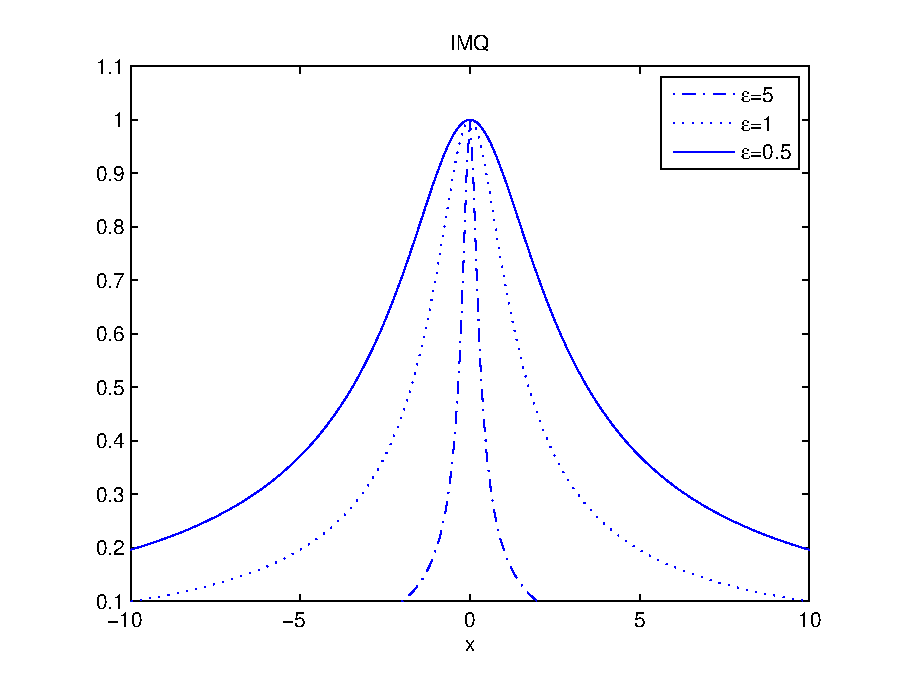
\includegraphics[height=5.5cm]{IMQ.eps}
		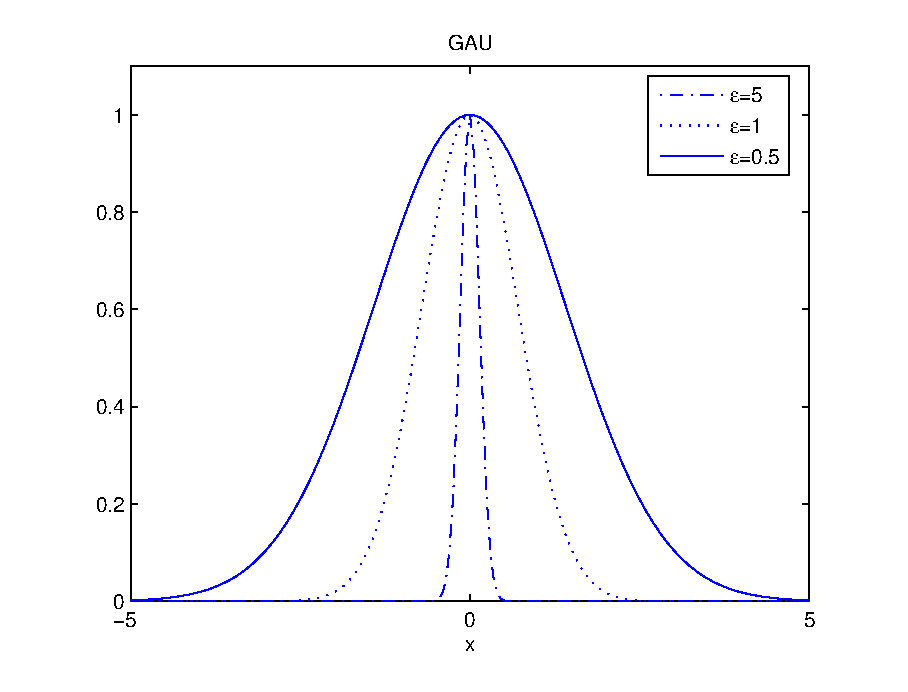
\includegraphics[height=5.5cm]{Gaussian.eps}}
	\centerline{
		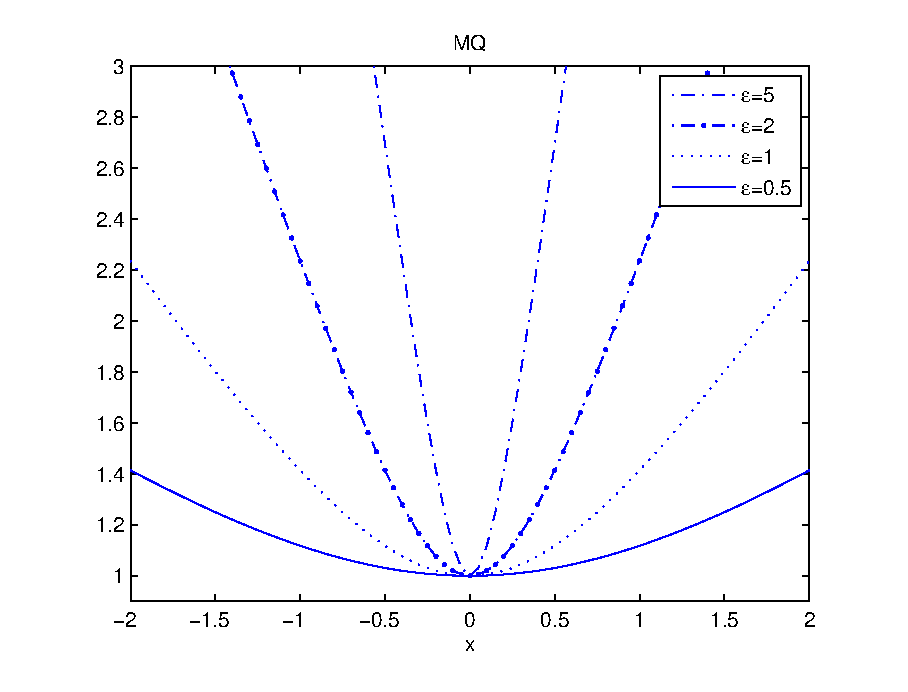
\includegraphics[height=5.5cm]{MQ.eps}
		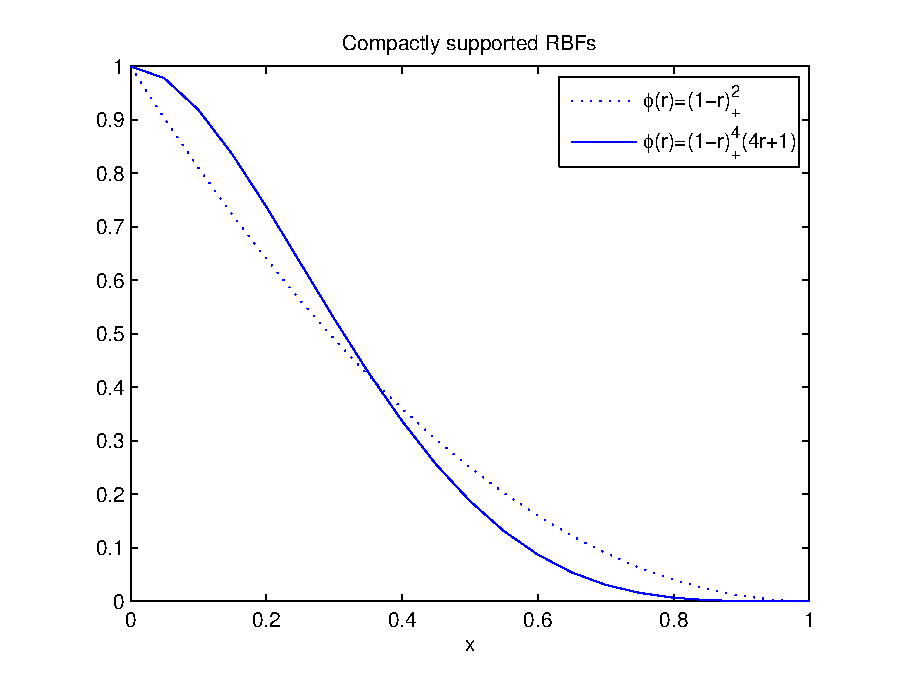
\includegraphics[height=5.5cm]{compact.eps}} 
	\caption{
		نمودار یک بعدی تعدادی از توابع پایه شعاعی با پارامتر پهناهای متفاوت}
	\label{fig:rbf}
\end{figure}
%


\section{درونیابی با توابع پایه شعاعی}
نقطه‌های متمایز 
$x_1,\ldots,x_N\in\mathbb{R}^d$
و مقدار تابع
$u(x_1),\ldots,u(x_N)$
متناظر با آن نقاط مفروض است. مساله استاندارد درونیابی با استفاده از توابع پایه شعاعی محاسبه  تابع درونیابی بصورت
\begin{equation}
	s(x)=\sum^{N}_{j=1}\lambda_j\phi(\|x-x_j\|)+p(x),\label{eq:int}
\end{equation}
است. که در آن
$\|.\|$
نرم اقلیدسی، 
$\lambda_j\in \mathbb{R}$, $j=1,\ldots,N$
ضرایب مجهول و 
$p\in\Pi^{d}_{m-1}$
فضای خطی تولید شده از چندجمله‌ای‌ها 
$d$
متغیره از درجه کوچکتر یا مساوی 
$m-1$
می‌باشد.

ماتریس 
$A\in{\mathbb {R}^{N\times N}}$
را بصورت 
$A_{ij}=\phi(\|x_i-x_j\|)$, $i,j=1,\ldots,N$
تعریف نموده  و فرض می‌کنیم
$\hat{m}$,
بعد فضای خطی 
$\prod^d_{m-1}$
باشد. بدیهی است که 
$\hat{m}=\binom{m+d-1}{d}$.
همچنین فرض کنید
$p_1,\ldots,p_{\hat {m} }$
پایه‌ای برای
$\prod^d_{m-1}$
باشد و ماتریس 
$P\in R^{N\times{\hat m}}$
را بفرم 
$P_{jk}=p_k(x_j)$, $k=1,\ldots,\hat{m}$, $j=1,\ldots,N$
تعریف می‌کنیم. ضرایب مجهول 
$\lambda_1,\ldots ,\lambda_N$ 
و
$\gamma_1,\ldots,\gamma_{\hat{m}}$
با اعمال شرایط درونیابی 
$s(x_j)=u(x_j)$, $j=1,\ldots,N$
و
$\sum_{j=1}^{N}\lambda_jp_k(x_j)=0$, $k=1,\ldots,\hat{m}$
حاصل می‌شود. اعمال این شرایط منجر به دستگاه خطی متقارن بلوکی بصورت زیر می‌شود.

\begin{equation}
	\begin{pmatrix}
		A & P  \\
		P^t & 0
	\end{pmatrix}
	\begin{pmatrix}
		\lambda \\
		\gamma
	\end{pmatrix}=
	\begin{pmatrix}
		u \\
		0
	\end{pmatrix},\label{mat:inter}
\end{equation}
که در آن   
$u=[u(x_1)\ldots u(x_N)]^T$, $\lambda=[\lambda_1\ldots\lambda_N]^T$ 
و
$\gamma=[\gamma_1\ldots \gamma_{\hat{m}}]^T$.

ماتریس متناظر با دستگاه 
(\ref{mat:inter}),
به ازای هر مجموعه از نقاط مجزای
$x_j$, $j=1,\ldots N$ 
معکوس پذیر است اگر و تنها اگر ماتریس 
$P$
رتبه کامل ستونی باشد
\citep{Micchelli}.
به همین دلیل 
$N\geq\hat{m}$
شرط لازم برای معکوس پذیری ماتریس ضرایب است.

اگر تابع 
$u$
هموار باشد و تابع پایه شعاعی هموار
$\phi$
برای درونیابی استفاده شود کاربر می‌تواند انتظار خطای خیلی کوچکی را داشته باشد.
\begin{definition}
	\citep{Wendland}
	برای یک دامنه کران‌دار 
	$\Omega$
	فاصله پرکننده
	بر مجموعه نقاط
	$X=\{x_1,\ldots,x_N\}\in\Omega$
	بصورت زیر تعریف می‌شود.
	\begin{equation*}
		h:=h_{X,\Omega}:=\sup_{x\in\Omega}\min_{1\leq j\leq N}\|x-x_j\|_2.
	\end{equation*}
\end{definition}
فاصله پرکننده را می‌توان فاصله حداکثری
$h$
تعبیر کرد که به ازای هر
$x\in\Omega$
یک نقطه 
$x_j$
با این فاصله موجود باشد.

در عمل هرگاه تراکم نقاط بیشتر شود، به عبارت دیگر
$h\rightarrow 0$
خطای درونیابی با استفاده از توابع پایه شعاعی همگرا به صفر می‌شود
\citep{Wu}.
برای توابع پایه شعاعی هموار از مرتبه بینهایت مانند توابع گاوسی و مالتی کوادراتیک معکوس حتی می‌توان همگرایی نمایی بفرم
$\exp^{(-c/h)}$
بدست آ ورد
\citep{Wendland}.
اما یک عامل بازدارنده جدی هنگام استفاده از توابع پایه شعاعی برای مجموعه نقاط چگال  یا بطور صحیح‌تر برای مجموعه نقاط با فاصله پرکننده کوچکتر وجود دارد. به عبارت دیگر، هرگاه فاصله جدا کننده 
\LTRfootnote{Separation distance}
کوچکتر شود، عدد حالت ماتریس ضرایب در 
(\ref{mat:inter})
به شدت افزایش می‌یابد.
\begin{definition}
	\citep{Larsson}
	برای دامنه کران‌دار
	$\Omega$
	فاصله جدا کننده برای مجموعه نقاط 
	$X=\{x_1,\ldots,x_N\}\in\Omega$
	بصورت زیر تعریف می‌شود.
	\begin{equation*}
		q_X:=\frac{1}{2}\min_{i\neq j}\|x_i-x_j\|_2.
	\end{equation*}
\end{definition}
فاصله جدا کننده را می توان ماکسیمم شعاع 
$r>0$
تعبیر کرد که گوی‌های 
$\{x \in \mathbb{R}^d: \|x - x _j\|_2 <r\}$
جدا از هم باشند.

مجموعه نقاط 
$X$
را یکنواخت گوسی
\LTRfootnote{Quasi-uniform}
نسبت به ثابت
$c > 1$
نامند هرگاه رابطه زیر برقرار باشد.
\begin{equation*}
	\frac{1}{c}q_X\leq h_{X,\Omega}\leq cq_X
\end{equation*}
وقتی که فاصله جدا کننده و  فاصله پرکننده متناسب باشند، ارتباط نزدیکی بین خطا و پایداری درونیابی وجود دارد. به عبارت دیگر ساختن تابع درونیابی از توابع پایه شعاعی که همزمان خطای خیلی کوچک با پایداری خوب را تضمین کند، وجود ندارد.



%										    %		اضافه نمودن فصل دوم

\chapter{روش هم‌محلی مبتنی بر توابع پایه شعاعی فراگیر  }\label{se:grbf}
%

در این فصل، روش هم‌محلی مبتنی بر توابع پایه شعاعی فراگیر برای حل عددی معادلات دیفرانسیل با مشتقات جزیی وابسته به زمان مورد مطالعه قرار می‌گیرد. جزییات این روش را با سه مثال ارایه خواهیم داد.



\section{شرایط مرزی چندگانه}
حالت یک بعدی معادلات روزنا را در بازه متقارن 
$[-L,\,L]$ 
بصورت
\begin{equation}
u_t+\alpha(x,t)u_{xxxxt}+\beta u_{xx}= g_u(u)u_x,\quad(x,t)\in
[-L,\,L]\times(0,\,T], \label{eq:Rosenau1D}
\end{equation}
با شرایط مرزی زیر است
\begin{align}
u(\pm L,t)&=f_1(\pm L,t),\quad t\in (0,\,T],\\
u_x(\pm L,t)&=f_2(\pm L,t),\quad t\in (0,\,T].\label{eq:1Dic}
\end{align}

در ادامه این رساله، فرض شده که
\begin{itemize}
\item
به ازای هر
$(x,t)\in\Omega\times[0,T]$
ثابت‌های مثبت
$\alpha_0$
و
$\beta_0$
وجود دارند بطوریکه

$\alpha_0<\alpha(x,t)<\beta_0$.

\item 
تابع $g$ را یک چندجمله‌ای از درجه 
$s+1$, $s>0$
در نظر می‌گیریم.
\end{itemize}
تا کنون، حتی برای حالت یک بعدی نیز هیچ روش مشخصی در هم‌محلی با توابع پایه شعاعی برای شرایط مرزی چندگانه در مسایل وابسته به زمان ارایه نشده است. در معادله
(\ref{eq:Rosenau1D})
دو شرط مرزی وجود دارد که باید در نقاط انتهایی دامنه صدق کنند. به عبارت دیگر، چهار شرط مرزی باید در دو نقطه مرزی صدق کنند. بنابراین، تعداد معادلات در هم‌محلی معادله 
(\ref{eq:Rosenau1D})
 در نقاط درونی بیشتر از تعداد نقاط خواهد بود. در واقع با یک دستگاه ابر معین سروکار خواهیم داشت که یا باید تعدادی از معادلات را کنار بگذاریم و یا باید تعدادی متغیر اضافی در نظر بگیریم.

تاکنون این طیف از مسایل در ادبیات روش‌های مبتنی بر توابع پایه شعاعی مطرح نشده است ولی در روش‌های هم‌محلی دیگری مانند روش‌های طیفی مورد بررسی قرار گرفته است. ما پنج روش که برای این نوع مسایل مورد بررسی قرار گرفته است را بصورت زیر لیست کرده‌ایم:
\begin{enumerate}
\item ترکیبی از شرایط مرزی ضعیف و سخت 
\item روش‌های جریمه‌ای طیفی 
\item تبدیل به دستگاه از مرتبه پایین‌تر 
\item روش نقطه تصوری
\item روش باز تصویر
\end{enumerate}
در این رساله، ما فقط روش‌های (3)-(5) را مورد مطالعه قرار می‌دهیم چرا که هیچ راهی برای پیدا کردن پارامتر جریمه که منجر به پایداری عددی جواب شود، برای روش‌های (1) و (2) وجود ندارد.

\subsection{تبدیل به دستگاه از مرتبه پایین‌تر}

از جمله روش‌های متداول برای حل معادلات دیفرانسیل با مشتقات از مرتبه بالاتر تبدیل به دستگاه معادلات دیفرانسیلی از مرتبه پایین‌تر می‌باشد. اگر قرار دهیم
$w = u_x$
آنگاه می‌توان معادله
(\ref{eq:Rosenau1D}) 
را بصورت زیر بازنویسی کرد.
\begin{align}
u_t + \alpha(x,t)w_{xxxt}+\beta w_x &= wg_u(u)\\
w_t - u_{xt} &= 0
\end{align}
که در آن 
$u(\pm L,t)=f_1(\pm L,t)$ 
و
$w(\pm L,t)=f_2(\pm L,t)$
شرایط مرزی هستند. 


مزیت این روش این است که شرایط مرزی نیومن
برای $u$ به شرایط مرزی دریکله
 برای $w$ تبدیل می‌شود ولی ابعاد دستگاه دو برابر می‌شود و حجم محاسبات بصورت قابل توجه افزایش می‌یابد. به همین دلیل، تبدیل به دستگاه از مرتبه پایین‌تر برای روش‌های مبتنی بر توابع پایه شعاعی فراگیر که ماتریس ضرایب پر هست، به صرفه نمی‌باشد. همچنین برای روش ‌هم‌محلی بر اساس توابع پایه شعاعی مبتنی بر تفاضلات متناهی که دارای ماتریس تنک می‌باشد، راه حل خوبی محسوب نمی‌شود. 

\subsection{روش نقطه تصوری}

تاکنون، روش‌های مبتنی بر نقطه تصوری برای اعمال شرایط مرزی چندگانه در روش تفاضلات متناهی مورد استفاده قرار گرفته است و اخیرا تعمیم آن برای روش‌های هم‌محلی فراگیر مانند روش‌‌های طیفی توسط فرنبرگ
مورد بررسی قرار گرفته است
\citep{Fornberg}.

 
 
\section{
پیاده سازی با
\textsc{متلب}}

در این بخش پیاده سازی روش نقطه تصوری و روش باز تصویر با متلب برای معادله روزنا ارایه شده است. همچنین برای نشان دادن جزییات بیشتر از پیاده سازی، برنامه‌های متلب روش‌های مطرح شده ارایه شده است.

\subsection{ پیاده سازی روش نقطه تصوری}

پیرو آنچه که در بخش‌های قبلی مربوط به روش نقطه تصوری گفته شد، دو نقطه مجازی به تعداد نقاط  گسسته شده اضافه نموده و ماتریس مشتق متناظر با تابع توسیع یافته‌ی پایه‌ مالتی‌کوادریک معکوس را ایجاد می‌کنیم. بعد از تفکیک ماتریس مشتق، می‌توان ماتریس 
$N-2\times N-2$
متناظر با نقاط درونی را بدست آورد. همچنین شرایط مرزی نیز توسط نقاط مرزی و نقاط تصوری اعمال می‌شود. سرانجام با به کاربردن روش ترازی می‌توان جواب تقریبی را محاسبه کرد.

کدهای ارایه شده معادله ارایه شده در 
(\ref{eq:Rosenau1D})-(\ref{eq:1Dic}) 
که دارای جواب دقیق 
$u(x,t)=\textnormal{sech}(x-t)$
می‌باشد؛ به ازای 
$g(u)=10u^3-12u^5-\frac{3}{2}u$, $\beta=0$, $\alpha(x,t)=1$ 
و 
$N=51$
نقطه گسسته شده با توزیع یکنواخت را در بازه
$[-1,1]$
حل می‌کند. دستگاه معادله دیفرانسیل معمولی حاصل با تابع
\textbf{ode15s}
متلب حل شده است.

\begin{latin} 	
\begin{verbatim}
    N = 51; L = 1; Tfinal = 30;
    phi = @(ep,r) 1./sqrt(1+(ep*r).^2); %Inverse MQ-RBF
    x = linspace(-1,1,N);
    linmap = @(x,x1,x2,y1,y2) (y2-y1)*(x-x1)/(x2-x1) + y1;
    % Map x to [-L,L] such that x(2) = -L, x(N-1) = L
    % and x(1), x(N) are left and right fictitious points respectively.
    x = linmap(x,x(2),x(N-1),-L,L); x = x(:); % RBF nodes
    ep = 0.1/min(diff(x)); % Shape parameter
\end{verbatim}
\end{latin} 	
که تابع
\textbf{odefun}
بصورت زیر است.
\begin{latin} 	
\begin{verbatim}
function U = odefun(t,u,x,N,D1d,D1bf,D4d,D4bf,Id)
    F = [sech(x([2 N-1]) - t); sech(x([2 N-1]) - t).*tanh(x([2 N-1]) - t)];
    Ft = [-sech(x([2 N-1]) - t).*tanh(x([2 N-1]) - t);...
end
\end{verbatim}
\end{latin}

\subsection{ پیاده سازی روش باز تصویر}

در بخش‌ مربوط به روش باز تصویر، چگونگی تبدیل معادله روزنا به دستگاه جبری دیفرانسیلی توضیح داده شد. به خاطر داریم که اعمال چهار شرط مرزی در نقاط مرزی منجر به چهار معادله جبری شد و  
$N-4$
معادله دیفرانسیلی نیز از هم‌محلی 
$N-4$
نقطه درونی کمکی ایجاد شد. همان طور که گفته شد نقاط کمکی نباید منطبق بر نقاط اصلی گسسته شده باشد.

فرض کنیم بردار
$u=[u_1 \cdots u_N]^T$
تقریب عددی جواب در نقاط
$x_1,\cdots,x_N $ 
باشد. حالت گسسته شده معادله با استفاده از روش باز تصویر را می‌توان بصورت ماتریسی و برداری زیر نشان داد.


\begin{latin}
\begin{verbatim}
    N = 51; L = 1; Tfinal = 30;
    phi = @(ep,r) 1./sqrt(1+(ep*r).^2); %Inverse MQ-RBF
    xc = linspace(-L,L,N).'; % RBF nodes
    ep = 0.1/min(diff(xc)); % Shape parameter
\end{verbatim}
\end{latin}
که تابع
\textbf{daefun} 
بصورت زیر است.
\begin{latin}
\begin{verbatim}
function F = daefun(t,u)
   u_t = (-1.5 - 60*u.^4 + 30*u.^2).*(D*u);
   BC = [u(1)-sech(xc(1)-t);u(N)-sech(xc(N)-t);...
end
\end{verbatim}
\end{latin}
%
%
\section{نتایج عددی}

در این بخش نتایج عددی حاصل از روش‌های باز تصویر و نقطه تصوری برای حل عددی معادله روزنا ارایه شده است. در این نتایج تابع چند مربعی معکوس بعنوان تابع پایه‌ای در نظر گرفته شده است. همچنین دامنه
$\Omega=[-15,15]$
با توزیع یکنواخت و توزیع نقاط هالتن گسسته سازی شده است.
%
\begin{figure}
\centerline{
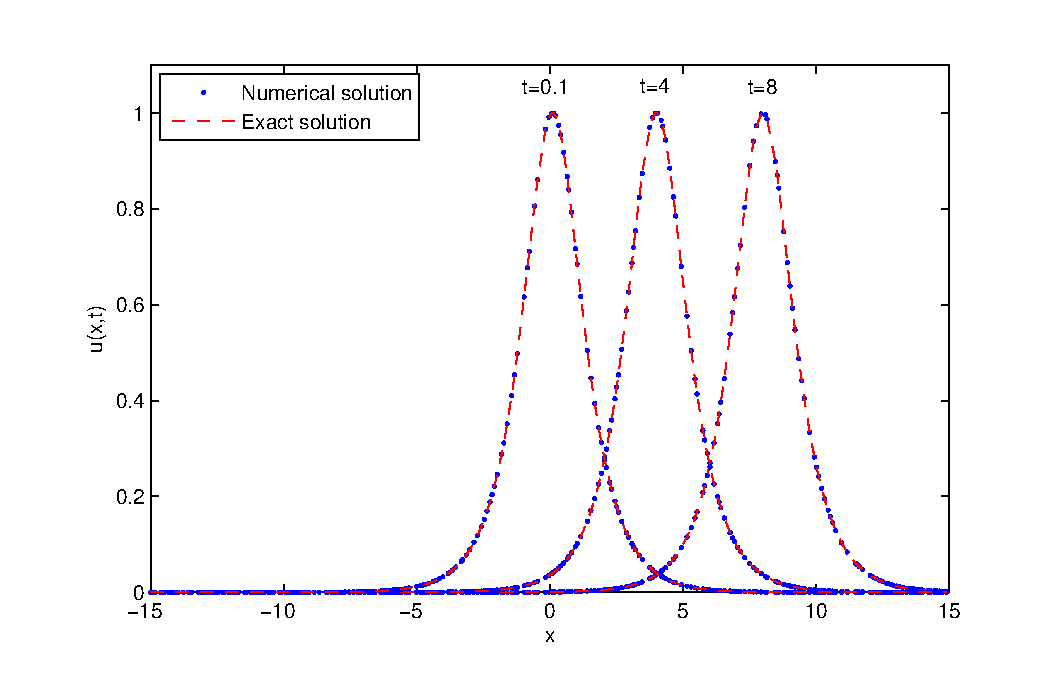
\includegraphics[height=7cm]{figure21.eps}} \caption{
جواب دقیق و تقریبی حاصل از روش باز تصویر به ازای 250 نقطه با توزیع هالتن و 
$\varepsilon=1$ } 
\label{fig:randpo}
\end{figure}
%
%
\begin{figure}
\centerline{
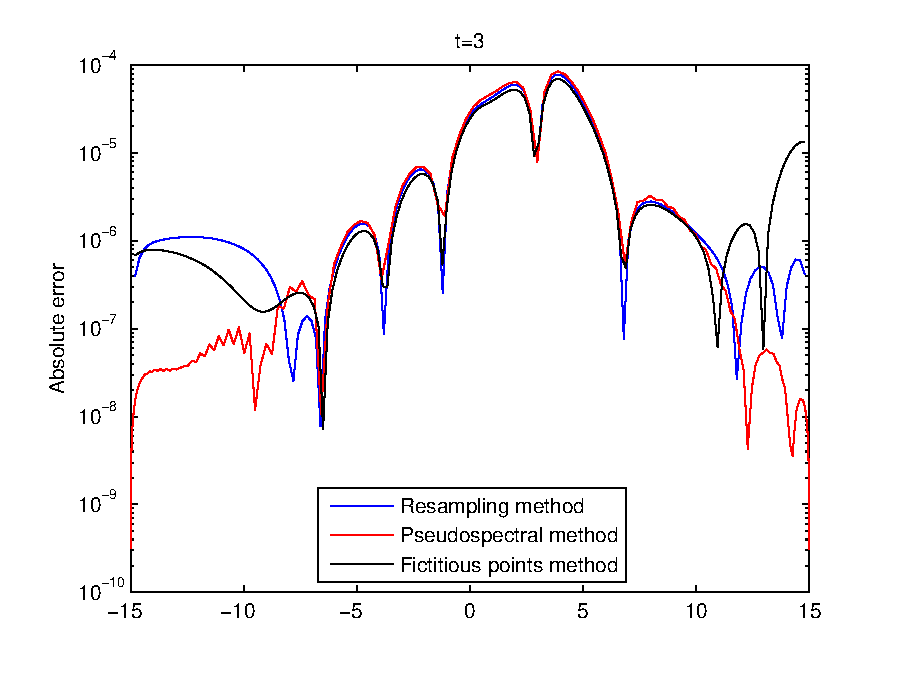
\includegraphics[height=6.5cm]{figure22.eps}
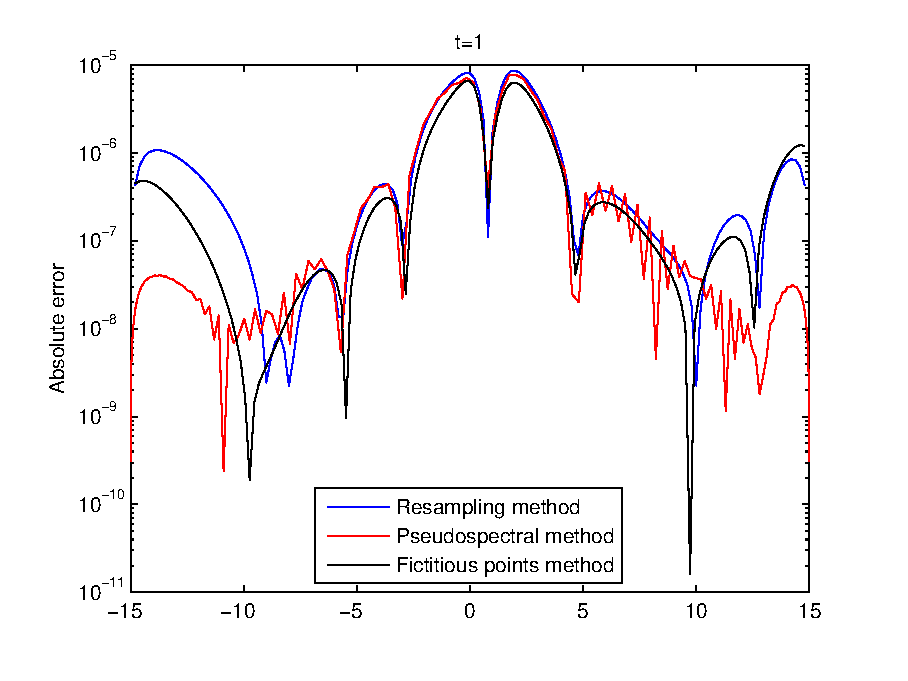
\includegraphics[height=6.5cm]{figure23.eps}} \caption{
مقایسه خطای مطلق روش باز تصویر و نقطه تصوری به ازای 150 نقطه یکنواخت و روش باز تصویر طیفی به ازای 150 نقطه چبیشف در 
$t=1$
و
$t=3$} \label{fig:absolute}
\end{figure}
%
%
معادله توسیع یافته روزنا که در مراجع
\citep{Wendland,ItoToi}
بیان شده است را در نظر می‌گیریم.
\begin{align}
u_t+\frac{1}{2}u_{xxxxt}=g(u)_x,\label{eq:test}
\end{align}
که
$g(u)=10u^3-12u^5-\frac{3}{2}u$.
جواب دقیق معادله
(\ref{eq:test})
بصورت
$u(x,t)=\textrm{sech}(x-t)$
می‌باشد. شرایط اولیه به ازای 
$t=0$
را می‌توان از جواب دقیق استخراج کرد.
\begin{align*}
u(x,0)=\textrm{sech}(x),
\end{align*}
همچنین شرایط مرزی نیز بفرم زیر است.
\begin{align*}
u(-15,t)&=\textrm{sech}(-15-t),&u&(15,t)=\textrm{sech}(15-t),\\
u_x(-15,t)&=-\textrm{sech}(-15-t)\textrm{tanh}(-15-t),&u_x&(15,t)=-\textrm{sech}(15-t)\textrm{tanh}(15-t).
\end{align*}
%
\begin{table}
\caption{ جواب تقریبی اختیار فروش امریکایی با دو دارایی پایه ناهمبسته با توزیع یکنواخت نقاط به ازای
 $\varepsilon=1.5$}
\label{tab:uinpoint}
\[\begin{array}{l@{\hspace{1cm}}c@{\hspace{1cm}}c@{\hspace{1cm}}c@{\hspace{1cm}}c}
\hline\noalign{\smallskip}
P(S_1,S_2,t) & 16 \times 16 \textrm{نقطه} & 21\times 21 \textrm{نقطه}
 & 31\times 31 \textrm{نقطه} & 41\times 41 \textrm{نقطه}  \\
\noalign{\smallskip}\hline\noalign{\smallskip}
  P(0.9,1,0)  & 7.8159e-002    & 7.4866e-002      &   7.6398e-002  &   7.5920e-002 \\
  P(1,0.9,0)  & 6.6373e-002    & 6.1842e-002      &   6.3400e-002  &   6.3700e-002 \\
  P(1,1.1,0)  & 3.1793e-002    & 3.1154e-002      &   3.2290e-002  &   3.2042e-002  \\
  P(1.1,1,0)  & 2.5447e-002    & 2.5159e-002      &   2.5865e-002  &   2.5925e-002 \\
\noalign{\smallskip}\hline
 \end{array}\]
\end{table}


\begin{table}
\centering{\caption{
خطای
$L_{\infty}$
حاصل از روش باز تصویر و نقطه تصوری به ازای 150 نقطه با توزیع یکنواخت و
$\varepsilon=0.5$
و خطای 
$L_{\infty}$
حاصل از روش باز تصویر طیفی به ازای 150 نقطه چبیشف
}}\label{tab:re1}
\vspace{-0.3cm}\begin{eqnarray*}\hspace{-0.2cm}\begin{array}{|c|c|c|c|c| } 
\hline {\rm \text{t} } &\hspace{2cm} {\rm
\text{باز‌تصویر}}
 &\hspace{2cm} {\rm \text{نقطه‌تصوری}} &\hspace{2cm} {\rm \text{باز‌تصویر‌طیفی}}\\
\hline
  0.1        &\hspace{2cm} 4.7842E^{-6}       &\hspace{2cm} 2.9565E^{-6}    &\hspace{2cm} 4.5572E^{-6}         \\
  0.5        &\hspace{2cm} 5.4018E^{-6}       &\hspace{2cm} 4.7338E^{-6}    &\hspace{2cm} 4.5603E^{-6}         \\
  1          &\hspace{2cm} 8.7933E^{-6}       &\hspace{2cm} 6.9239E^{-6}    &\hspace{2cm} 7.6580E^{-6}         \\
  3          &\hspace{2cm} 8.1032E^{-5}       &\hspace{2cm} 7.3506E^{-5}    &\hspace{2cm} 8.4876E^{-5}         \\
  5          &\hspace{2cm} 2.6041E^{-4}       &\hspace{2cm} 2.4963E^{-4}    &\hspace{2cm} 2.8425E^{-4}         \\
  8          &\hspace{2cm} 6.9731E^{-4}       &\hspace{2cm} 2.0524E^{-3}    &\hspace{2cm} 7.8322E^{-4}         \\
  10         &\hspace{2cm} 1.0868E^{-3}       &\hspace{2cm} 1.5169E^{-2}    &\hspace{2cm} 1.2464E^{-3}        \\
  \hline
 \end{array}\end{eqnarray*}
\end{table}

\begin{table}[htp] 
\centering\caption{
خطای
$L_{\infty}$
حاصل از روش باز تصویر و نقطه تصوری به ازای 150 نقطه با توزیع یکنواخت و
$\varepsilon=0.5$
و خطای 
$L_{\infty}$
حاصل از روش باز تصویر طیفی به ازای 150 نقطه چبیشف
}
\label{tab:re1}
\renewcommand*{\arraystretch}{1.2}
\vspace*{.4cm}
%\begin{LTR}
\begin{tabular}{||c|c|c|c||}%{|c@{\hspace{10mm}}|c@{\hspace{10mm}}|c@{\hspace{10mm}}|c@{\hspace{10mm}}|}
%{||c|c|c|c||}
\hline
$t$ & باز تصویر &  طیفی  & باز تصویر طیفی   \\
\hline
0.1     & 4.7842   & 2.9565     & 4.5572        \\
  0.5        & 5.4018       & 4.7338    & 4.5603        \\
  1          & 8.7933      &6.9239     & 7.6580        \\
  3          & 8.1032       & 7.3506   & 8.4876       \\
  5          & 2.6041      &2.4963    & 2/8425        \\
  8          &6.9731     & 2.0524     & 7.8322       \\
  10         & 1.0868      & 1.5169     & 1.2464      \\
\hline
\end{tabular}
%\end{LTR}
\end{table}
%
%
	                                        %		اضافه نمودن فصل سوم

\chapter{روش‌های هم‌محلی موضعی مبتنی بر توابع پایه شعاعی  }\label{se:rbfloc}
%
در فصل قبل، روش هم‌محلی توابع پایه شعاعی برای معادلات دیفرانسیل با مشتقات جزیی وابسته به زمان مورد مطالعه قرار گرفت. در این فصل، فرمولبندی دیگری از توابع پایه شعاعی که منجر به درونیابی موضعی با نقاط پراکنده  می‌شود، مورد بررسی قرار می‌گیرد. برخلاف روش‌های فراگیر، درونیابی موضعی منجر به ماتریس ضرایب تنک می‌شود. در این فصل، در حالت کلی دو روش موضعی به شرح زیر بررسی خواهد شد.

\begin{enumerate}
\item توابع پایه شعاعی مبتنی بر تفاضلات متناهی
\item روش توابع پایه شعاعی مبتنی افراز واحد
\end{enumerate}

\section{روش افراز واحد}	                                        %		اضافه نمودن فصل چهارم
%\chapter{
اختیار خرید آمریکایی 
}
\label{se:option}
%
در فصل‌های سوم و چهارم نشان داده شد که توابع پایه شعاعی از دقت بالایی برای تقریب مسایل چند بعدی برخوردار هستند. همچنین نشان داده شد که روش‌های مبتنی بر بدون شبکه‌بندی بصورت قابل توجهی حجم محاسبات را کاهش می‌دهد. بنابراین این‌گونه روش‌ها بعنوان روشی کارا برای حل مسایل مالی محسوب می‌شوند. تقریب عددی اختیار خریدهای اروپایی و آمریکایی در حالت یک بعدی، اولین بار توسط 
\citep{Hon,McLain}
مورد بررسی قرار گرفت. 
\citep{Pettersson}،
اختیار خریدهای چند بعدی را مورد تقریب عددی قرار دادند. اختیار خرید‌های اروپایی و آمریکایی در حالت یک و دو بعدی توسط 
\citep{Fasshauer}
مورد مطالعه قرار گرفت. در همه مطالعات فوق الذکر که برای حل عددی اختیار خریدها انجام شده، توابع پایه شعاعی در حالت موضعی به کار گرفته شده است. همانطور که در فصل قبل ذکر شد؛ توابع پایه شعاعی مبتنی بر افراز واحد یک روش موضعی است که منجربه تقریب‌های با دقت بالا و ماتریس‌های تنک می‌شود که مناسب برای مسایل چند بعدی است.

در این فصل، اختیار خریدهای چندبعدی را در نظر می‌گیریم و روش توابع پایه شعاعی مبتنی بر افراز واحد را برای بررسی عددی این نوع مسایل به کار می‌بریم.

                                         %		اضافه نمودن فصل پنجم
%
\chapter{نتيجه‌گيری و پیشنهادهای آتی}
\label{se:Conclusion}

در این پایان‌نامه توابع پایه شعاعی بعنوان یک روش کارا برای حل عددی معادلات دیفرانسیل با مشتقات جزیی وابسته به زمان مورد استفاده قرار گرفته‌اند. نتایج بدست آمده را می‌توان بصورت زیر بیان کرد:
\begin{enumerate}
\item 
روش هم‌محلی مبتنی بر توابع پایه شعاعی فراگیر منجر به تقریب با دقت بهتری در مقایسه با روش‌های کرنک-نیکلسون و روش عناصر متناهی می‌باشد. 
\item 
فصل پنجم این رساله پیاده سازی روش توابع پایه شعاعی مبتنی بر روش افراز واحد برای تقریب جواب اختیار خرید دوبعدی آمریکایی را مورد بررسی قرار داده و جزییات محاسباتی آن را بیان می‌کند.
\end{enumerate}
به عنوان پیشنهاد برای کارهای آینده به موارد زیر اشاره می‌کنیم:
\begin{enumerate}
\item
تعمیم روش توابع پایه شعاعی فراگیر به مسایل معکوس.
\item
بررسی پایداری روش‌های توابع پایه شعاعی مبتنی بر افراز واحد و تفاضلات متناهی.
\item
ایجاد تابعی برای حل عددی معادلات دیفرانسیل با مشتقات جزیی وابسته به زمان با استفاده از توابع پایه شعاعی.
\end{enumerate}                                  %		اضافه نمودن فصل نتیجه گیری
%                                         ------------------------------------------------------------------
%			  		                نام فایل هر قسمت از ضمیمه را به صورت جداگانه وارد کنید
% 
\appendix
\doublespacing
\setlength{\baselineskip}{1\baselineskip}
\chapter{کدهای زبان برنامه‌نویسی\lr{Python}}


% دستورات زیر برای زیبایی کدها در قسمت پیوست می‌باشد.
\lstset{  
	basicstyle=\ttfamily, 
	numbers=left,                   
	numberstyle=\tiny\color{blue},  
	stepnumber=1,                
	numbersep=5pt,                
	backgroundcolor=\color{gray!10},  
	showspaces=false,              
	showstringspaces=false,        
	showtabs=false,                
	rulecolor=\color{black},         
	tabsize=2,                     
	captionpos=b,                   
	breaklines=true,                
	breakatwhitespace=false,        
	keywordstyle=\color{purple},      
	commentstyle=\color{green},  
	stringstyle=\color{red}{ForestGreen}      
}

در این قسمت کدهای مربوط به نرم افزار شما قرار دارد.
\begin{latin}
	\begin{lstlisting}[language=Python, caption={Example Python code}]
	# Import Libraries
	import numpy as np
	import matplotlib.pyplot as plt
	
	x = np.linspace(0, 2*np.pi, 100)
	y = np.sin(x)
	plt.plot(x, y)
	\end{lstlisting}
\end{latin}

							    	%		اضافه نمودن ضمیمه 
%                                      -----------------------------------------------------------------------
%
                                      %    مقالات مستخرج از پایان نامه 	خود را در این قسمت وارد کنید.
\doublespacing 
%
\chapter*{مقالات مستخرج از پایان‌نامه}
\addcontentsline{toc}{chapter}{مقاله‌های مستخرج از پایان‌نامه}
\vspace{.5cm}

 
\begin{latin}
\begin{enumerate}
%
\item  {A. Golbabai, A. Safdari-Vaighani},
\textit{ A meshless method for numerical solution of the coupled Schrodinger-KdV equations},
{ Computing, 92 (2011), pp. 225–242}.



\item  {A. Golbabai, A. Safdari-Vaighani},
\textit{Collocation method based on radial basis function for the coupled Klein-Gordon-Schrodinger equations},
{Electronic Transactions on Numerical Analysis, 39 (2012), pp. 22-31.}


\item {A. Golbabai, A. Safdari Vaighani},
\textit{Width optimization of Gaussian function by genetic algorithm in RBF networks},
{World Journal of Modelling and Simulation, 7 (2011), pp. 307-311. }

\item {A. Golbabai, A. Safdari Vaighani},
\textit{Global optimization of expensive functions with mixed-integer constrained using radial basis functions},
{the 40 th Iranian International Conference on Mathematics 20-24 Agust  2009,  Sharif University of Technology, Tehran, Iran.}

\item {A. Golbabai, A. Safdari Vaighani},
\textit{A meshless method for the numerical solution of the two-dimensional Zakharov-Kuznetsov equation},
{the 2th Annual Iranian applied Mathematics March  2010,  Sistan and Blochestan University, Zahedan, Iran.}

\item {A. Golbabai, A. Safdari Vaighani},
\textit{Approximate solution of the KGS equation using RBF in a finite-Difference mode},
{the 41th Iranian International Conference on Mathematics 12-15 September 2010, University of Urmia, Urmia, Iran.}


\end{enumerate}
\end{latin}

                                                      %مراجع با یکی از سه روش زیر ایجاد می شود.
                                                                      %توجه   توجه   توجه
                 %(براي ايجاد ارجاها بصورت پارانتر به جاي كروشه به سطر 16-18 فایل  commands مراجعه کنید).
%%%%%%%%%%%%%%%%%%%%%%%%%%%%%%%%%%%%%%%%%%%%%%%%%
%% 1- برای ایجاد مرجع‌ها با شماره دو سطر زیر را فعال کنید  (الگوی گروه رياضي).
%\bibliographystyle{plain-fa}%{asa-fa}%      مرجع‌ها%
%\bibliography{MyReferences}
% 2- برای ایجاد مرجع‌ها با اسامی و سال دو سطر زیر را فعال کنید  (الگوی گروه آمار).
\bibliographystyle {asa-fa}% {unsrt-fa}%   مرجع‌ها%
\bibliography{MyReferences}
                                                                           
% 3- برای ایجاد مرجع‌ها با شماره سطر زیر را فعال کنید (بدون ايجاد فابل بيب)
%%
%
%														پس از اضافه نمودن مراجع، این فایل را ذخیره نموده و سپس فایل اصلی رساله را اجرا کنید
%
%
\begin{thebibliography}{99} 						
%
\begin{latin} 	


\bibitem{[68]} {\sc M.A. Abdou, A.A. Soliman},  {\em New applications of variational iteration
method},  Physica D: Nonlinear Phenomena, 211 (2005), pp. 161-182.

\bibitem{[69]} {\sc K. Appert, J. Vaclavik}, {\em Dynamics of coupled solitons}, Phys. Fluids., 20 (1977), pp.
1845-1849.

\bibitem{[15]} {\sc I. Babu$\check{s}$ka , J. M. Melenk}, {\em The partition of unity method}, Int. J. Numer.
Methods Eng., 40 (1997), 727-758.

\bibitem{[63]} {\sc A. Bachelot},  {\em Probleme de Cauchy pour des systems hyperboliques semi-lineaires}, Ann. Inst. Henri
Poincaré Anal. Non Linéaire, 1 (1984), pp. 453-478.

\bibitem{[70]} {\sc D. Bai, L. Zhang}, {\em The finite element method for the coupled Schr\"{o}dinger-KdV
equations}, Physics Letters A., 373 (2009),  2237-2244.

\bibitem {[67]} {\sc W. Bao and L. Yang}, {\em Efficient and accurate numerical methods for the Klein-Gordon-Schr\"{o}dinger equations},
J. Comput. Phys., 225 (2007), pp. 1863-1893.

\bibitem {[25]} {\sc W. Bao and L. Yang}, {\em Efficient and accurate numerical methods for the Klein-Gordon-Schr\"{o}dinger equations},
J. Comput. Phys., 225 (2007), pp. 1863-1893.

\bibitem {[34]} {\sc J. P. Boyd}, {\em Error saturation in Gaussian radial basis function on a finite interval},
J. Comput. Appl. Math., 234 (2010), pp. 1435-1441.

\bibitem{[3]} {\sc M.D. Buhmann}, {\em A new glass of radial basis functions
with compact support}, Mathematices of computation, 70 (2000),
307-318.

\bibitem{[4]} {\sc A. H.-D. Cheng, M. A. Golberg, E. J. Kansa, and G.
Zammito}, {\em Exponential convergence and h-c multiquadric
collocation method for partial differential equations}, Numer.
Methods Partial Differential Equations, 19 (2003), pp. 571-594.

\bibitem {[82]} {\sc S.M. Choo, S. K. Chung, K. I. Kim}, {\em A discontinuous Galerkin
 method for the Rosenau equation}, Applied Numerical Mathematics, 58 (2008), pp. 783-799.

\bibitem{[46]} {\sc S. K. Chung, S. N. Ha},
{\em Finite element Galerkin solutions for the Roseneau equation},
Applic. Analysis., 54 (1994), pp. 39-56.

\bibitem{[5]} {\sc T. A. Driscoll and B. Fornberg}, { \em Interpolation in the limit of increasingly flat
radial basis functions}, Comput. Math. Appl., 43 (2002), pp.
413-422.

\bibitem{[51]} {\sc D. Duffie}, {\em Dynamic Asset Pricing Theory}, Princeton
University Press, 1996.

\bibitem {[76]} {\sc G. E. Fasshauer}, {\em Meshless methods}, In Handbook of Theoretical
and Computational Nan-otechnology, American Scientic publishers,
2005.

\bibitem{[53]}{\sc G. Fasshauer, A.Q.M. Khaliq, D.A. Voss}, {\em Using mesh free
approximation for multi asset American options},  Journal of
Chinese Institute of Engineers, 27 (2004), pp. 563-571.

\bibitem {[30]} {\sc B. Fornberg}, {\em Calculation of weights in finite
difference formulas}, SIAM Reviews, 40 (1998), pp. 685-691.

\bibitem{[80]} {\sc B. Fornberg}, {\em A pseudospectral fictitious point method for high order
initial-boundary value problems}, SIAM J. Sci. Comput., 28 (2006), pp.
1716-1729.

\bibitem{[43]} {\sc B. Fornberg, G.B. Whitham}, {\em Anumerical and theoretical study of certain nonlinearwave phenomena},
Philos Trans. R. Soc., 289 (1978), pp. 373-404.

\bibitem{[74]} {\sc R. Frank}, {\em Scattered data interpolation: Tests of
some methods}, mathematics of computation, 38 (1982), pp. 181-200.

\bibitem{[75]} {\sc R. Franke, G. Neilson}, {\em Smooth interpolation of large
sets of scattered data}, J. Numer. Methods Eng.,  15 (1980), pp.
1691-1704.

\bibitem{[61]} {\sc I. Fukuda and M. Tsutsumi}, {\em On coupled Klein-Gordon-Schr\"{o}dinger equations
 II}, J. Math. Anal. Appl., 66 (1978), pp. 358-378.

\bibitem{[64]} {\sc I. Fukuda and M. Tsutsumi},  {\em On coupled Klein-Gordon-Schr\"{o}dinger equations
III}, Math. Jpn., 24 (1979), pp. 307-321.

\bibitem {[20]} {\sc B. Guo, L. Shen}, {\em In: Proceedings Of DD-3 Symposium},
Chang chun., 417 (1982).

\bibitem{[55]} {\sc Y.C. Hon, X.Z. Mao}, {\em A radial basis function method for solving options pricing
models}, J. Financial Engineering, 8 (1999), pp. 31-49.

\bibitem{[81]}{\sc Y. C. Hon and R. Schaback}, {\em On unsymmetric
collocation by radial basis functions}, Appl. Math. Comput., 119
(2001), pp. 177-186.

\bibitem{[18]} {\sc F. T. Hioe}, {\em Periodic solitary waves for two coupled nonlinear Klein-Gordon and Schr\"{o}dinger equations}, J. Phys. A: Math. Gen., 36
(2003), pp. 7307-7330.

\bibitem{[48]} {\sc B. Hu, Y. Xu and J. Hu}, {\em Crank-Nicolson finite difference scheme for the
Rosenau-Burges equation}, Appl. Math. Comput., 204 (2008), pp.
311-316.

\bibitem{[66]} {\sc W. Jia, L. Biao and Y. Wang-Chuan}, {\em Approximate solution for the Klein-Gordon-Schr\"{o}dinger
equation by the homotopy analysis method}, Chin. Phys. B., 19
(2010), pp. 30401-7.

\bibitem{[77]} {\sc E.J. Kansa} {\em Multiquadrics-a  scattered data approximation scheme with
applications to computational fluid dynamics}, Comput. Math.
Appl., 19 (1990), pp. 127-145.

\bibitem{[78]} {\sc E.J. Kansa}, {\em Motivation for using radial basis
functions to solve PDEs}, Tech. rep., Lawrence Livermore
Laboratory (1999).

\bibitem{[71]} {\sc D. Kaya, M. El-Sayed} {\em On the solution of the coupled Schr\"{o}dinger-KdV equation
by the decomposition method}, Physics Letters A., 313 (2003), pp.
82-88.

\bibitem{[52]} {\sc Y.K. Kwok}, {\em Mathematical Models of Financial Derivatives}, Springer-Verlag, 1998.

\bibitem{[57]} {\sc A.Q.M. Khaliq, D.A. Voss, and S.H.K. Kazmi}, {\em Linearly implicit penalty
methods for pricing American options}, Western Illinois
University, preprint 2003.

\bibitem{[42]} {\sc A.J. Khattak,
Siraj-ul-Islam}, {\em A comparative study of numerical solutions
of a class of KdV equation}, Appl. Math. Comp.,  199 (2008) pp.
425-434.

\bibitem{[90]} {\sc A. Larsson, A. Heryudono}, {\em Radial basis function based on partition of unity method in irregular geomerty domains}, to prepare.

\bibitem{[47]} {\sc H.Y. Lee, M.J. Ahn},
{\em The convergence of the fully discrete solution for the
Roseneau equation}, Computers Math. Appl., 32 (1996), pp. 15-22.

\bibitem{[8]} {\sc W.R. Madych, S.A. Nelson}, {\em Bounds on multivariate polynomials and exponential error
estimates for multiquadric interpolation}, J. Approx. Theory., 70
(1992) pp. 94-114.

\bibitem{[14]} {\sc D.H. McLain}, {\em Two dimensional interpolation from random data}, Comput.
J., 19 (1976), pp. 178-181.

\bibitem{[16]}  {\sc C.A. Micchelli},  {\em Interpolation of scatterded data:
distance matrix and conditionally positive definite functions},
Constr. Approx., 2 (1986), pp. 11-22.

\bibitem{[58]} {\sc B.F. Nielsen, O. Skavhaug, and A. Tveito},
{\em Penalty methods for the numerical solution of American
multi-asset option problems}, Department of Informatics,
University of Oslo, 2000.

\bibitem{[59]} {\sc B.F. Nielsen, O. Skavhaug, and A.
Tveito}, {\em Penalty and front-fixing methods for the numerical
solution of American option problems}, J. Comput. Finance., 5
(2002), pp. 69-97.

\bibitem{[44]} {\sc M.A. Park}, {\em Model equations in fluid dynamics}, Ph. D. Dissertation,
Tulane University, 1990.

\bibitem {[45]} {\sc M.A. Park}, {\em Pointwise decay estimates of solutions of the
generalized Rosenau equation}, J. of Korean Math. Soc., 29 (1992),
pp. 261-280.

\bibitem{[56]} {\sc U. Pettersson, E. Larsson, G. Marcusson and J. Persson}, {\em Improved radial basis function methods for
multi-dimensional option pricing}, Journal of Computational and
Applied mathematics, 222 (2008), pp. 82-93.

\bibitem{[6]} {\sc S. Rippa}, {\em An algorithm for selecting a good value for the parameter c in radial
basis function interpolation}. Adv. Comput. Math., 11 (1999), pp.
193-210.

\bibitem{[41]} {\sc P. Rosenau}, {\em Dynamics of dense discrete systems}, Prog. Theoret.
Phys., 79 (1988), pp. 1028-1042.

\bibitem{[72]} {\sc R. Schaback}, {\em Kernel-Based Meshless Methods}, hand
book, 2007.

\bibitem{[10]} {\sc R. Schaback}, {\em Error estimates and condition numbers for radial
basis function interpolation}, Adv. Comput. Math., 3 (1995) pp.
251–264.

\bibitem {[33]} {\sc R. Schaback and H. Wendland}, {\em Kernel techniques: From machine learning to meshless methods},
Acta Numerica, 15 (2006), pp. 543-639.

\bibitem{[13]} {\sc D. Shepard}, {\em A two dimensional interpolation function for irregularly spaced
data}, In Proceedings of the ACM national conference, (1968), pp.
517-524.

\bibitem{[12]} {\sc C. Shu, H. Ding and K. S. Yeo}, {\em Local radial basis
function-based differential quadrature method and its application
to solve two-dimensional incompressible Navier-Stokes equations},
Comput. Method. Appl. M., 192 (2003), pp. 941-954.

\bibitem{[73]} {\sc N. Tanaka}, {\em Development of a highly accurate
interpolation method for mesh-free flow simulations I, integration
of a gridless particle and CIP methods}. International Journal for
Numerical method in Fluids, 30 (1999), pp. 957-976.

\bibitem{[50]} {\sc D. Tavella, C. Randall}, {\em Pricing Financial Instruments}, Wiley (New York),
2000.

\bibitem {[65]} {\sc M. L. Wang and Y. B. Zhou}, {\em The periodic wave solutions for the Klein-Gordon-Schr\"{o}dinger
equations},  Phys. Lett. A., 318 (2003), pp. 84-92.

\bibitem{[9]} {\sc H. Wendland}, {\em Scattered Data Approximation}, Cambridge University Press, 2005.

\bibitem{[2]} {\sc H. Wendland}, {\em Piecewise polynomial, positive definite
and compactly supported radial functions on minimal degtee},
Advanced in Computational Mathematics, 4 (1995), pp. 389-396.

\bibitem{[11]} {\sc G. B. Wright and B. Fornberg}, {\em Scattered node compact
finite difference-type formulas generated from radial basis
functions}, J. Comput. Phys., 212 (2006), pp. 99-123.

\bibitem{[1]} {\sc Z. Wu}, {\em Compactly supported positive definite radial
basis functions}, Advanced in computational Mathematics, 4 (1995),
pp. 283-292.

\bibitem{[54]} {\sc Z. Wu, Y.C. Hon}, {\em Convergence error estimate in solving free
boundary diffusion problem by radial basis functions method},
Engrg. Anal. Bound. Elem., 27 (2003), pp. 73-79.

\bibitem{[7]} {\sc J. Yoon}, {\em Spectral approximation orders of radial basis function interpolation on the Sobolev
space}. SIAM J. Math. Anal., 33 (2001), pp. 946-958.

\bibitem {[62]} {\sc H. Yukawa}, {\em On the interaction of elementary particles I}, Proc.
PhysicoMath. Soc. Japan., 17 (1935), pp. 48-57.

\bibitem{[49]} {\sc K. Zheng, J. Hu}, {\em Crank-Nicolson difference scheme for the
generalized Rosenau-Burgers equation}, International Journal of
Applied Mathematics and Computer Sciences, 5 (2009), pp. 252-256.

\bibitem{[60]} {\sc R. Zvan, P.A. Forsyth and K. R. Vetzal}, {\em Penalty methods for American options
with stochastic volatility}, Comput. Appl. Math., 91 (1998), pp.
199-218.
\end{latin} 	
\end{thebibliography}            	                	%		 مرجع‌ها
%%%%%%%%%%%%%%%%%%%%%%%%%%%%%%%%%%%%%%%%%%%%%%%%%%%%

\chapter*{واژه‌نامه فارسی به انگلیسی}\markboth{واژه‌نامه فارسی به انگلیسی}{واژه‌نامه فارسی به انگلیسی} 
\addcontentsline{toc}{chapter}{واژه‌نامه فارسی به انگلیسی}
%\thispagestyle{empty}
ا\\
\englishgloss{Probabilistic}{احتمالی}
\englishgloss{Valuation}{ارزیابی}
\englishgloss{Measure}{اندازه }
پ\\
\englishgloss{Stably}{پایدار}
ت\\
\englishgloss{Weak Topology}{توپولوژی ضعیف}
د\\
\englishgloss{Powerdomain}{دامنه‌توانی}
\englishgloss{Semantic Domain}{دامنه معنایی}
م\\
\englishgloss{Dcpo}{مجموعه جزئاً مرتب کامل جهت‌دار}
\englishgloss{Ordered}{مرتب}						    	    	 %		واژه‌نامه انگلیسی به فارسی

                                           % براي ايجاد نمايه سه سطر زير را فعال نماييد.        
%\refstepcounter{chapter}
%\addcontentsline{toc}{chapter}{نمایه}
%\printindex									        	%		دستور ظاهر شدن نمایه‌ها

\doublespacing
\setlength{\baselineskip}{1\baselineskip}
%
%
%														پس از اضافه نمودن خلاصه انگلیسی، این فایل را ذخیره نموده و سپس فایل اصلی رساله را اجرا کنید
%
%
\thispagestyle{empty} 	%		prevents tex from numbering of this page
\begin{latin} 					% 	xepersian enviorment
	
	\centerline{\textbf{\large{Abstract}}}
	\vskip 1cm
	\noindent 
	In this thesis, we invistigate the global RBF collocation method
	for the non-linear system of the time-dependent PDEs. Even for the
	one-dimensional case, how to implement multiple boundary
	conditions for a time-dependent problem is not obvious. We explore
	this difficulty and possible remedies at theoretical and practical
	levels. Theoretically, we study the error estimate of global RBF
	collocation method when the method of line is applied  for
	discretized form of the time-dependent non-linear PDEs.
	Computationally, we present the details of implementation for the
	new proposed methods. The efficiency of the proposed methods is
	demonstrated by comparing with the other methods.
	We also study the local RBF collocation methods for numerical
	solution of the PDEs. The partition of unity based on RBF is
	introduced as a robust method for the time-dependent PDEs. The
	properties of the partition of unity method (PUM) allow to have
	greater flexibility to adjust local approximation. We generate the
	differentiation matrices based on RBF--PUM discretizations and
	show that such schemes can lead to sparse matrices that is
	suitable for numerical study of the large scale problems. 
	As a more practical approach, we develop the RBF--PUM
	for the numerical approximation of the two-dimensional American
	put option pricing.\\
	
	\noindent
	\textbf{Keywords:} 
	\emph{PDEs, Radial basis function, Partition of unity method, collocation method, Error estimate.}
\end{latin}						        	% 	چکیده انگلیسی
\singlespacing
%
%
%                                                                               توجه
%											             	در این فایل تغییر نیاز نیست بدهید

\thispagestyle{empty}
\begin{center}
	\begin{latin}
		
\includegraphics[width=35mm]{enatu.jpg} \\
		\begin{Large}
		\enuniversity \\
		\enDep \\
		\enmajor \\[5 mm]
		\enlevel\  \\
		\end{Large}
		\vskip .8cm
		\large{Title}      \\[2mm] \textbf{\huge{\entitle}}
		\vskip 1cm
		\large{Supervisor} \\[2mm] \Large{\ensupervisor}
	    \vskip 8mm
		\large{Advisor} \\[2mm] \Large{\enadvisor}
		    \vskip 10mm
		\large{Examiner} \\[2mm] \Large{\enreferee}
				\vskip 8mm
			\large{By}          \\[2mm] \Large{\enAuthor}
		\vskip 12mm
		\large{\engdate}
	\end{latin}
\end{center}							        	%		روی جلد انگلیسی
%
\end{document}
